\documentclass[fleqn,10pt]{physiome}
% Use option lineno for line numbers 

\articletype{Review}
%% Choose from Original, Retrospective, Review, Letter

\title{The Boron \& De Weer Model of Intracellular pH Regulation}

\author[1][rxo22@case.edu]{Rossana Occhipinti}
\author[2]{Soroush Safaei}
\author[2]{Peter J. Hunter}
\author[1,3]{Walter F. Boron}
\affil[1]{Department of Physiology and Biophysics, Case Western Reserve University, School of Medicine, Cleveland, OH 44106, USA}
\affil[2]{Auckland Bioengineering Institute, University of Auckland, Auckland, New Zealand}
\affil[3]{Departments of Medicine and Biochemistry, Case Western Reserve University, School of Medicine, Cleveland, OH 44106, USA}

%% The following lines can be omitted when submitting;
%% information will be added by editors
\publicationdate{27 August 2020}
\editor{Karin Lundeng\r{a}rd}
\curator{Anand K. Rampadarath}
\submitteddate{25 August 2020}
\accepteddate{25 August 2020}
\citethisas{Occhipinti et al. (2020)\\The Boron & De Weer Model of Intracellular pH Regulation. Physiome.}{10.36903/physiome.12859469}

\begin{document}

\maketitle

\begin{abstract}
The classic \cite{boron1976intracellular} paper provided the first evidence of active regulation of $\mathrm{pH}$ in cells by an energy-dependent acid-base transporter. These authors also developed a quantitative model --- comprising passive fluxes of acid-base equivalents across the cell membrane, intracellular reactions, and an active transport mechanism in the cell membrane (modelled as a proton pump) --- to help interpret their measurements of intracellular $\mathrm{pH}$ under perturbations of both extracellular $\mathrm{CO_2}/\mathrm{HCO_3^-}$ and extracellular $\mathrm{NH_3}/\mathrm{NH_4^+}$. This \emph{Physiome} paper seeks to make that model, and the experimental conditions under which it was developed, available in a reproducible and well-documented form, along with a software implementation that makes the model easy to use and understand. We have also taken the opportunity to update some of the units used in the original paper, and to provide a few parameter values that were missing in the original paper. Finally, we provide an historical background to the \cite{boron1976intracellular} proposal for active $\mathrm{pH}$ regulation and a commentary on subsequent work that has enriched our understanding of this most basic aspect of cellular physiology. 
\end{abstract}

\keywords{$\mathrm{CO_2}$, $\mathrm{NH_3}$, squid giant axon, weak acid, weak base}

\primarypubs[10.36903/physiome.12859469]{bibliography}{boron1976p}

\section{Introduction}

In 1976 Boron \& De Weer published their landmark paper on ``Intracellular $\mathrm{pH}$ transients in squid giant axons caused by $\mathrm{CO_2}$, $\mathrm{NH_3}$, and metabolic inhibitors'' \citep{boron1976intracellular}. The authors used a squid giant axon preparation and a mathematical model of $\mathrm{pH}$ buffering and the transport of protons, bicarbonate ($\mathrm{HCO_3^-}$) and $\mathrm{CO_2}$ to establish the experimental evidence for active regulation of intracellular $\mathrm{pH}$ ($\mathrm{pH_i}$) by a transporter in the plasma membrane that --- at the expense of energy --- either moves acid out of the cell, or base into the cell. Today, we refer to such a transporter generically as an acid-extrusion mechanism. For simplicity, Boron \& De Weer modelled it as a proton pump, although the result would have been almost indistinguishable had they modelled it as the uptake of $\mathrm{HCO_3^-}$ or carbonate ($\mathrm{CO_3^{2-}}$). The paper reported on the consequences of adding and then removing extracellular $\mathrm{CO_2}/\mathrm{HCO_3^-}$, $\mathrm{NH_3/NH_4^+}$ (where $\mathrm{NH_4^+}$ is ammonium), or the metabolic inhibitors, cyanide, azide and dinitrophenol (DNP).

In the first experiment, following exposure of the cell to elevated $\mathrm{CO_2}$ and $\mathrm{HCO_3^-}$, $\mathrm{CO_2}$ rapidly enters the cell and intracellular $\mathrm{CO_2}$ equilibrates with the extracellular $\mathrm{CO_2}$, and generates intracellular $\mathrm{H^+}$ and $\mathrm{HCO_3^-}$ via the $\mathrm{CO_2}$ hydration reaction ($\mathrm{CO_2}+\mathrm{H_2O} \longrightarrow \mathrm{H^+}+\mathrm{HCO^-_3}$). The accumulating $\mathrm{H^+}$ results in a rapid fall of $\mathrm{pH_i}$ (see \autoref{fig:1}A \& \autoref{fig:1}B). To the extent that the membrane is permeable to $\mathrm{HCO_3^-}$ as well as to $\mathrm{CO_2}$, $\mathrm{HCO_3^-}$ will initially enter the cell passively, along its electrochemical gradient. Soon, however, the accumulation of intracellular $\mathrm{HCO_3^-}$ reverses the $\mathrm{HCO_3^-}$ electrochemical gradient and would be expected to lead to the passive efflux of $\mathrm{HCO_3^-}$. This loss of cellular $\mathrm{HCO_3^-}$ would tend to acidify the cell because --- to replenish the lost $\mathrm{HCO_3^-}$ --- additional $\mathrm{CO_2}$ would enter the cell and form even more $\mathrm{H^+}$ and $\mathrm{HCO_3^-}$ (the passive $\mathrm{CO_2}/\mathrm{HCO_3^-}$ shuttle). Thus, the expectation was that prolonged exposure to $\mathrm{CO_2}$ would cause $\mathrm{pH_i}$ to fall rapidly (passive influx of $\mathrm{CO_2}$) and then to drift more slowly in the acidic direction (passive efflux of $\mathrm{HCO_3^-}$). In fact, Boron \& De Weer observed an \textit{alkaline} drift, leading to the postulate of active extrusion of $\mathrm{H^+}$ --- or an equivalent process\footnote{Of course, other energy-requiring processes --- as yet undiscovered at the time --- could also have accounted for the $\mathrm{pH_i}$ increase.} --- at a rate that exceeds the passive shuttling by the $\mathrm{CO_2}/\mathrm{HCO_3^-}$ couple (see \autoref{fig:1}A \& \autoref{fig:1}C).

\begin{figure}[ht]
\centering
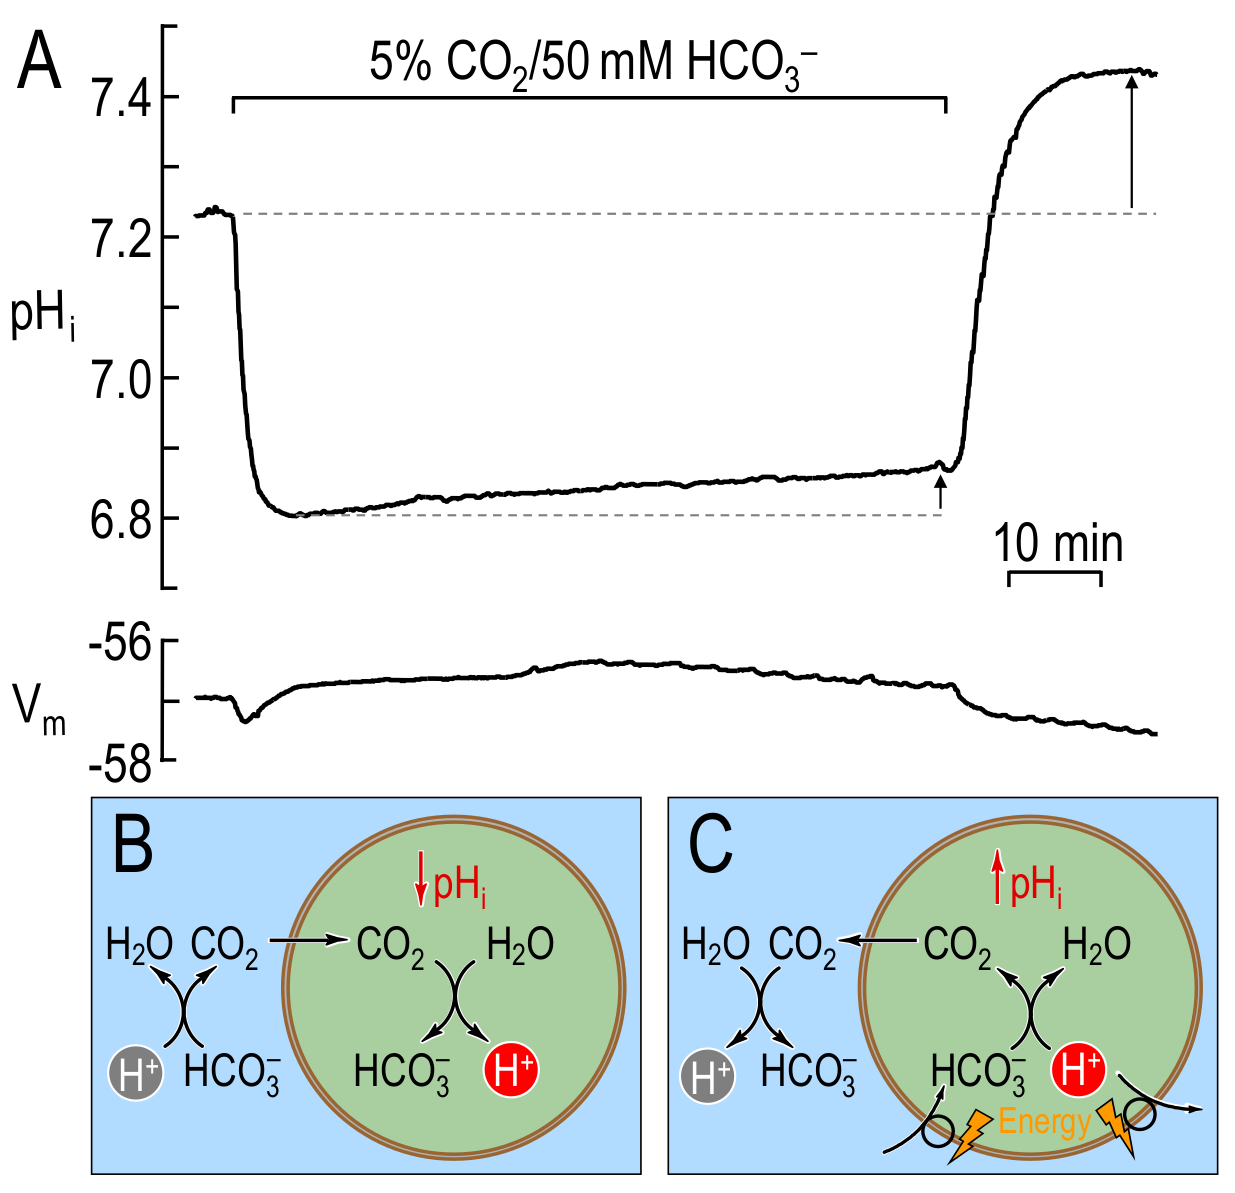
\includegraphics[width=0.49\linewidth]{img/Figure 1.png}
\caption{\label{fig:1} $\mathrm{pH_i}$ changes caused by prolonged exposure of a squid giant axon to extracellular $\mathrm{CO_2}/\mathrm{HCO_3^-}$ in the bulk solution. \textbf{(A)} Original $\mathrm{pH_i}$ and $V_\mathrm{m}$ traces from figure 1 of BDW. Exposing an axon to extracellular $\mathrm{CO_2}/\mathrm{HCO_3^-}$ causes a rapid fall in $\mathrm{pH_i}$ followed by a slow and sustained plateau-phase $\mathrm{pH_i}$ recovery (\emph{i.e.}, $\mathrm{pH_i}$ rises). Removing extracellular $\mathrm{CO_2}/\mathrm{HCO_3^-}$ causes $\mathrm{pH_i}$ to overshoot its initial resting value. Both the plateau-phase recovery (short arrow) and the overshoot (long arrow) are indicative of net acid extrusion during the period of $\mathrm{CO_2}/\mathrm{HCO_3^-}$ exposure. \textbf{(B)} Cartoon illustrating the processes underlying the initial, rapid acidification phase in (A). The entry of $\mathrm{CO_2}$ leads to the intracellular production of $\mathrm{H^+}$ (and thus to the observed $\mathrm{pH_i}$ decay) via the reaction $\mathrm{CO_2}+\mathrm{H_2O} \longrightarrow \mathrm{H^+}+\mathrm{HCO^-_3}$. \textbf{(C)} Cartoon illustrating the processes underlying the plateau-phase alkalinisation in (A). After $\mathrm{CO_2}$ equilibration across the plasma membrane ($\mathrm{pH_i}$ nadir in panel (A)), the slow entry of $\mathrm{HCO_3^-}$ (or, equivalently, the slow exit of $\mathrm{H^+}$) --- which has always been present but was overwhelmed by the influx of $\mathrm{CO_2}$ --- leads to the consumption of $\mathrm{H^+}$ (and thus to the observed slow $\mathrm{pH_i}$ rise) via the reaction $\mathrm{H^+}+\mathrm{HCO^-_3} \longrightarrow \mathrm{CO_2}+\mathrm{H_2O}$. The newly formed $\mathrm{CO_2}$ then exits the cell. The observed $\mathrm{pH_i}$ overshoot is the result of the accumulation of $\mathrm{HCO_3^-}$ during exposure to extracellular $\mathrm{CO_2}/\mathrm{HCO_3^-}$. BDW used the mathematical model to postulate the presence of an active acid-extrusion mechanism that would explain both the observed plateau-phase $\mathrm{pH_i}$ recovery and the $\mathrm{pH_i}$ overshoot. (A), modified from \cite{boron1976intracellular}. (B)-(C), modified from \cite{boron2010sharpey}.}
\end{figure}

Following removal of external $\mathrm{CO_2}$, intracellular $\mathrm{CO_2}$ diffuses out, while intracellular $\mathrm{HCO_3^-}$ combines with $\mathrm{H^+}$ to leave the cell as $\mathrm{CO_2}$. Thus, the entire intracellular $\mathrm{H^+}$ load associated with $\mathrm{CO_2}$ entry would be removed, returning $\mathrm{pH_i}$ to its value before the addition of $\mathrm{CO_2}/\mathrm{HCO_3^-}$ (or to a slightly lower value, to the extent that $\mathrm{HCO_3^-}$ had passively exited during the $\mathrm{CO_2}/\mathrm{HCO_3^-}$ exposure). In fact, Boron \& De Weer observed that $\mathrm{pH_i}$ overshoots its resting value by an amount consistent with the net removal of $\mathrm{H^+}$ by the active, acid-extrusion mechanism during the $\mathrm{CO_2}/\mathrm{HCO_3^-}$ exposure (see \autoref{fig:1}A \& \autoref{fig:1}C).

In the second experiment, following exposure of the cell to extracellular $\mathrm{NH_3}/\mathrm{NH_4^+}$ in the form of $\mathrm{NH_4Cl}$ (ammonium chloride), the intracellular environment rapidly becomes alkaline as $\mathrm{NH_3}$ enters and combines with $\mathrm{H^+}$ to form $\mathrm{NH_4^+}$ (equivalent to the hydration of $\mathrm{NH_3}$ to form $\mathrm{NH_4^+}$ and $\mathrm{OH^-}$). If this were the entire story, then $\mathrm{pH_i}$ would rise monotonically to a relatively alkaline value, and then the subsequent removal of $\mathrm{NH_4Cl}$ would cause $\mathrm{pH_i}$ to fall to precisely its initial value. In fact, Boron \& De Weer observed that the exposure to $\mathrm{NH_4Cl}$ causes $\mathrm{pH_i}$ to rise rapidly and then fall slowly. Moreover, the subsequent removal of $\mathrm{NH_3}/\mathrm{NH_4^+}$ causes $\mathrm{pH_i}$ to undershoot its original value (see \autoref{fig:2}A). Thus, Boron \& De Weer postulated that, during the $\mathrm{NH_3}/\mathrm{NH_4^+}$ exposure, $\mathrm{NH_4^+}$ passively enters the cell down its electrochemical gradient. Early during the exposure, this $\mathrm{NH_4^+}$ influx would oppose the $\mathrm{NH_3}$ entry and slightly reduce the $\mathrm{pH_i}$ increase. Later during the $\mathrm{NH_4Cl}$ exposure, after intracellular $\mathrm{[NH_3]}$ rises to match extracellular $\mathrm{[NH_3]}$ ($\mathrm{[NH_3]_o}$), the continued passive influx of $\mathrm{NH_4^+}$ would generate intracellular $\mathrm{H^+}$ and $\mathrm{NH_3}$. The result would be a slow fall of $\mathrm{pH_i}$ and a rise in intracellular $\mathrm{[NH_3]}$, the latter leading to the passive exit of $\mathrm{NH_3}$ (the passive $\mathrm{NH_3}/\mathrm{NH_4^+}$ shuttle, see \autoref{fig:2}A \& \autoref{fig:2}B). The experimental data are consistent with the proposed mathematical model.

\begin{figure}[ht]
\centering
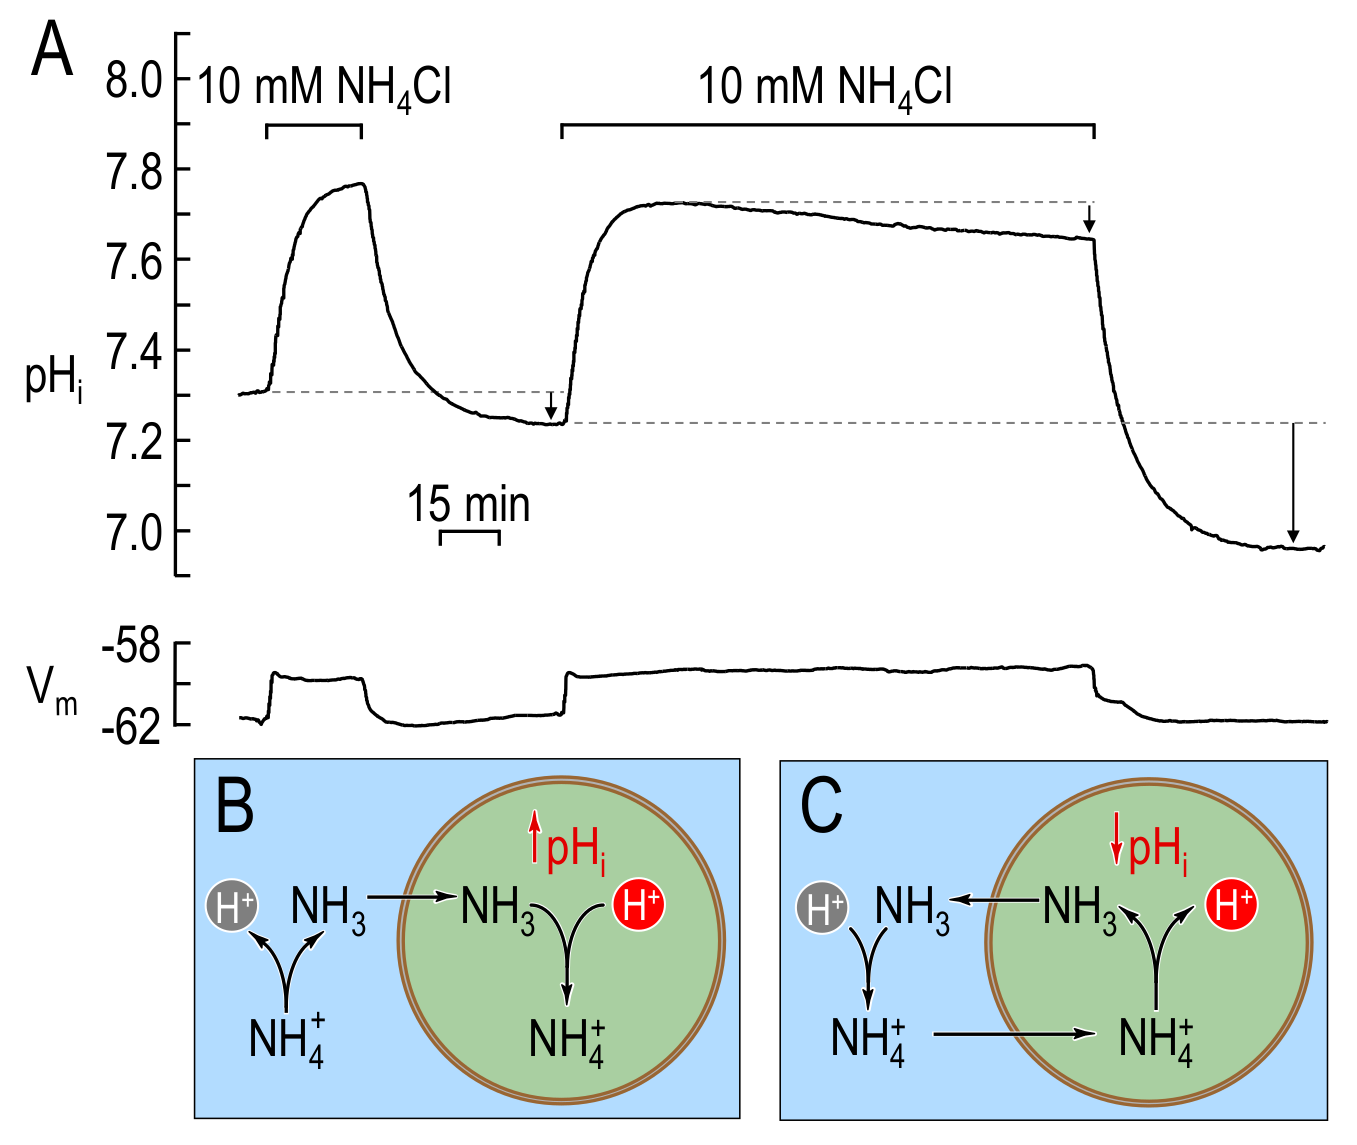
\includegraphics[width=0.49\linewidth]{img/Figure 2.png}
\caption{\label{fig:2} $\mathrm{pH_i}$ changes caused by a short and a long exposure of a squid giant axon to extracellular $\mathrm{NH_3}/\mathrm{NH_4^+}$ in the bulk solution. \textbf{(A)} Original $\mathrm{pH_i}$ and $V_\mathrm{m}$ traces from figure 2 of BDW. A short exposure of the axon to extracellular $\mathrm{NH_3}/\mathrm{NH_4^+}$ causes a rapid rise in $\mathrm{pH_i}$, followed by a $\mathrm{pH_i}$ decay that modestly undershoots (lower short arrow) its initial resting value upon removal of extracellular $\mathrm{NH_3}/\mathrm{NH_4^+}$. A longer exposure of squid giant axons to extracellular $\mathrm{NH_3}/\mathrm{NH_4^+}$ causes a rapid rise in $\mathrm{pH_i}$, followed by a slow and sustained $\mathrm{pH_i}$ decay. Removing extracellular $\mathrm{NH_3}/\mathrm{NH_4^+}$ causes $\mathrm{pH_i}$ to undershoot substantially its initial resting value (long arrow). Both the plateau-phase acidification (upper short arrow) and the undershoot (long arrow) are indicative of net acid loading during the period of $\mathrm{NH_3}/\mathrm{NH_4^+}$ exposure. \textbf{(B)} Cartoon illustrating the processes underlying the initial alkalinisation phase in (A) for both short and long exposures to extracellular $\mathrm{NH_3}/\mathrm{NH_4^+}$. The initial entry of $\mathrm{NH_3}$ leads to the intracellular consumption of $\mathrm{H^+}$ (and thus to the observed $\mathrm{pH_i}$ rise) via the reaction $\mathrm{NH_3}+\mathrm{H^+} \longrightarrow \mathrm{NH^+_4}$. \textbf{(C)} Cartoon illustrating the processes underlying the plateau-phase acidification during the long $\mathrm{NH_3}/\mathrm{NH_4^+}$ exposure in (A). After $\mathrm{NH_3}$ equilibration across the plasma membrane ($\mathrm{pH_i}$ peak in panel (A)), the slow entry of $\mathrm{NH_4^+}$ --- which has always been present but overwhelmed by the influx of $\mathrm{NH_3}$ --- leads to the production of $\mathrm{H^+}$ (and thus to the observed slow $\mathrm{pH_i}$ decay during the plateau phase) via the reaction $\mathrm{NH^+_4} \longrightarrow \mathrm{NH_3}+\mathrm{H^+}$. The newly formed $\mathrm{NH_3}$ then exits the cell. The $\mathrm{pH_i}$ undershoots observed upon removal of extracellular $\mathrm{NH_3}/\mathrm{NH_4^+}$, during both short and long $\mathrm{NH_3}/\mathrm{NH_4^+}$ exposures, are the result of the accumulation of $\mathrm{NH_4^+}$ during exposure to extracellular $\mathrm{NH_3}/\mathrm{NH_4^+}$. BDW used the mathematical model to postulate the above sequence of events, including both the plateau-phase acidification and the $\mathrm{pH_i}$ undershoot. (A), modified from \cite{boron1976intracellular}. (B)-(C), modified from \cite{boron2010sharpey}.}
\end{figure}

Finally, exposure of the cells --- in turn --- to cyanide, DNP and azide resulted in intracellular acidosis, consistent with the accumulation of acid metabolites.

In the present paper, we re-formulate the models from \cite{boron1976intracellular}, henceforth referred to as `BDW', and specify the simulation using the Physiome modelling standards CellML \citep{cuellar2003overview} and SED-ML \citep{bergmann2017sed} in order to ensure that the model reproduces the graphs in the original paper and that the model is fully curated.\footnote{\url{https://models.physiomeproject.org/workspace/5f8}} Note that this effort requires the specification of some parameters used in BDW's simulations, but not described in the BDW paper. The curated and annotated model is made available in a form that users can run with OpenCOR\footnote{\url{http://www.opencor.ws}} to understand the model and to explore the effect of changes in parameter values.

\section{pH Buffering by Weak Acids and Weak Bases}

We begin by reviewing a few rudimentary concepts of $\mathrm{pH}$ buffering by weak acids and bases \citep{roos1981intracellular,bevensee2013control,boron2016medical} to provide the background for understanding the derivation and implementation of the BDW model.

\paragraph{Buffers.}

According to Br\"{o}nsted's definition \citep{bronsted1923einige}, an acid is any substance that can donate a $\mathrm{H^+}$. Conversely, a base is any substance that can accept a $\mathrm{H^+}$. A buffer is any substance that can reversibly consume or produce $\mathrm{H^+}$, thereby minimising changes in $\mathrm{pH}$.

The dissociation of the uncharged weak acid ($\mathrm{HA}$) to the anionic weak base ($\mathrm{A^-}$) is described by the equilibrium reaction:
\begin{equation}
\mathrm{HA \rightleftharpoons A^- + H^+}
\end{equation}
which is governed by the equilibrium constant\footnote{Note that $\mathrm{[A^-]}$ denotes a concentration in units of $\mathrm{mol\cdot m^{-3}}$ or $\mathrm{mM}$.}
\begin{equation}
K_\mathrm{HA}=\dfrac{\mathrm{[A^-][H^+]}}{\mathrm{[HA]}}.
\label{eqn:K_A}
\end{equation}
An example is the carbonic acid ($\mathrm{H_2CO_3}$) dissociation reaction,
\begin{equation*}
\mathrm{H_2CO_3 \rightleftharpoons HCO_3^- + H^+}.
\end{equation*}
The total weak acid concentration, $\mathrm{[TA]}$, is the sum of $\mathrm{[HA]}$ and $\mathrm{[A^-]}$. Note that $\mathrm{[TA]}$ is one of the two main unknowns in the BDW model for weak acids.

The dissociation of the cationic weak acid ($\mathrm{BH^+}$) to the uncharged weak base ($\mathrm{B}$) is described by the equilibrium reaction,
\begin{equation}
\mathrm{BH^+ \rightleftharpoons B + H^+},
\end{equation}
where the equilibrium constant is
\begin{equation}
K_\mathrm{BH}=\dfrac{\mathrm{[B][H^+]}}{\mathrm{[BH^+]}}.
\end{equation}
An example is the $\mathrm{NH_4^+}$ dissociation reaction,
\begin{equation*}
\mathrm{NH_4^+ \rightleftharpoons NH_3 + H^+}.
\end{equation*}
The total weak base concentration, $\mathrm{[TB]}$, is the sum of $\mathrm{[BH^+]}$ and $\mathrm{[B]}$. Note that $\mathrm{[TB]}$ is one of the two main unknowns in the BDW model for weak bases.

\paragraph{The $\mathrm{CO_2}/\mathrm{HCO_3^-}$ buffer pair.}

The formation of $\mathrm{HCO_3^-}$ and $\mathrm{H^+}$ from $\mathrm{CO_2}$ by hydration is given by the equilibrium reaction
\begin{equation*}
\mathrm{CO_2 + H_2O \rightleftharpoons HCO_3^- + H^+},
\end{equation*}
where the equilibrium constant is
\begin{equation}
K_\mathrm{CO_2}=\dfrac{\mathrm{[HCO_3^-][H^+]}}{\mathrm{[CO_2]}}.
\label{eqn:KCO2}
\end{equation}
Taking logarithms of both sides of \autoref{eqn:KCO2}, and recognising from Henry's law that
\begin{equation}
\mathrm{[CO_2]}=s\cdot p_\mathrm{CO_2},
\end{equation}
where $s$ is the solubility coefficient for $\mathrm{CO_2}$ and $p_\mathrm{CO_2}$ is the partial pressure of $\mathrm{CO_2}$, we obtain the familiar Henderson-Hasselbalch equation
\begin{equation}
\mathrm{pH}=\mathrm{pK_{CO_2}}+\log{\dfrac{\mathrm{[HCO_3^-]}}{s\cdot p_\mathrm{CO_2}}}.
\end{equation}
Here, $\mathrm{pH}=-\log[\mathrm{H^+}]$\footnote{The definition of $\mathrm{pH}$ as a $\mathrm{pH}$ scale based on powers of 10 was introduced by S{\o}rensen in an attempt to simplify the notation of $\mathrm{[H^+]}$ and to avoid having to resort to decimals for tiny amounts of $\mathrm{[H^+]}$ \citep{sorensen2007messung}.} and $\mathrm{pK_{CO_2}}=-\log(K_\mathrm{CO_2})$.

In terms of the nomenclature above, one might regard $\mathrm{CO_2}$ as the weak acid $\mathrm{HA}$\footnote{Note that although $\mathrm{CO_2}$ is often regarded as an acid, the true weak acid is $\mathrm{H_2CO_3}$, the product of the reaction of $\mathrm{CO_2}$ with $\mathrm{H_2O}$.}, and $\mathrm{HCO_3^-}$ as its conjugate base $\mathrm{A^-}$.

\paragraph{Buffering power ($\beta$).}

By definition, $\beta$ is the amount of strong base (\emph{e.g.}, $\mathrm{NaOH}$), or the negative of the amount of strong acid (\emph{e.g.}, $\mathrm{HCl}$), that one must add to $1~\mathrm{L}$ of solution to raise $\mathrm{pH}$ by one $\mathrm{pH}$ unit:
\begin{equation}
\beta=\dfrac{\Delta\text{[Strong~Base]}}{\Delta \mathrm{pH}}=-\dfrac{\Delta\text{[Strong~Acid]}}{\Delta \mathrm{pH}}.
\label{eqn:buffer}
\end{equation}
The units of $\beta$ are $\mathrm{mM}$. For additional details, refer to \cite{roos1981intracellular,boron2016medical}. Note that BDW defined $\beta$ as a negative number, as did Koppel and Spiro in their original definition of buffering \citep{koppel1914wirkung,roos1980buffer}, rather than as a now-conventional positive quantity, as did Van Slyke in his later work \citep{van1922measurement}. BDW's definition, which they consistently applied, has no effect on the outcome of their simulations. In the present paper, we will follow the definition of Van Slyke --- defining $\beta$ as a positive number --- and make appropriate sign changes to the derived equations.

\section{The Boron \& De Weer Model for the Permeation by an Uncharged Weak Acid and its Conjugate, Anionic Weak Base}

The BDW mathematical model consists of two time-dependent ordinary differential equations (ODEs), one describing the time-course of the concentration of total intracellular buffer ($\mathrm{[TA]_i} = \mathrm{[HA]_i}+\mathrm{[A^-]_i}$) and the other the time-course of the intracellular free $\mathrm{H^+}$ concentration (which is related to $\mathrm{pH_i}$). BDW derived these two equations for the general cases in which any buffer pair $\mathrm{HA}/\mathrm{A^-}$, or any buffer pair $\mathrm{B}/\mathrm{BH^+}$, can move passively across the plasma membrane of a prototype cell. Then, they applied these two general equations to their specific experimental conditions, namely exposure of a cell (a squid giant axon) to equilibrated extracellular $\mathrm{CO_2}/\mathrm{HCO_3^-}$ or to equilibrated extracellular $\mathrm{NH_3}/\mathrm{NH_4^+}$.

Here, following BDW's approach, we begin by deriving the equations for $\mathrm{HA}/\mathrm{A^-}$. In the next section, we apply the same general formalism to $\mathrm{B}/\mathrm{BH^+}$.

\paragraph{Derivation for weak acids.}

Imagine that a cell is exposed to a solution containing equilibrated $\mathrm{HA}/\mathrm{A^-}$ and that both $\mathrm{HA}$ and $\mathrm{A^-}$ initially move into the cell --- because of the chemical gradient in the case of $\mathrm{HA}$, and because of the electrochemical gradient in the case of $\mathrm{A^-}$.

An integrated form of Fick's first law of diffusion describes the net passive influx\footnote{BDW used $M$ to denote a transmembrane flux. In the present paper, we use the more widely used notation $J$.} of $\mathrm{HA}$ ($J_\mathrm{HA}$)
\begin{equation}
J_\mathrm{HA}=P_\mathrm{HA}\bigg(\mathrm{[HA]_o}-\mathrm{[HA]_i}\bigg),
\label{eqn:J_HA}
\end{equation}
where $J_\mathrm{HA}$ is flux ($\mathrm{mol\cdot m^{-2}\cdot s^{-1}}$) and $P_\mathrm{HA}$ ($\mathrm{m\cdot s^{-1}}$) is the membrane permeability to the uncharged weak acid $\mathrm{HA}$. Note that this is a passive diffusion equation because $\mathrm{HA}$ is uncharged.

The constant field equation --- also known as the Goldman, Hodgkin, Katz (GHK) \citep{goldman1943potential,hodgkin1952quantitative} equation --- describes the net passive influx of $\mathrm{A^-}$ ($J_\mathrm{A^-}$):
\begin{equation}
J_\mathrm{A^-}=P_\mathrm{A^-}\left(\dfrac{V_\mathrm{m}F}{RT}\right)\left(\dfrac{\mathrm{[A^-]_o}-\epsilon\mathrm{[A^-]_i}}{1-\epsilon}\right),
\label{eqn:J_A}
\end{equation}
where $P_\mathrm{A^-}$ ($\mathrm{m\cdot s^{-1}}$) is the membrane permeability to the charged conjugate base $\mathrm{A^-}$, $V_\mathrm{m}$ is the membrane potential (intracellular relative to extracellular potential), and $\epsilon$ is a shorthand for $e^{{-V_\mathrm{m}F}/{RT}}$. Note that $J_\mathrm{HA}$ and $J_\mathrm{A^-}$ have units of $\mathrm{mol\cdot m^{-2}\cdot s^{-1}}$.

Although $\mathrm{HA}$ and $\mathrm{A^-}$ can interconvert in the cytosol, BDW assumed that the intracellular concentration of total weak acid $\mathrm{[TA]_i}$ only can change due to the transmembrane fluxes of $\mathrm{HA}$ and $\mathrm{A^-}$ (see \autoref{fig:3}). Thus, the time rate of change of $\mathrm{[TA]_i}$ is
\begin{equation}
\dfrac{\mathrm{d[TA]_i}}{\mathrm{d}t}=\rho\left(J_\mathrm{HA}+J_\mathrm{A^-}\right),
\label{eqn:TArate}
\end{equation}
where $\rho$ ($\mathrm{m^{-1}}$) is the area-to-volume ratio for the cell, and converts the transmembrane flux per unit area (in units of $\mathrm{mol\cdot m^{-2}\cdot s^{-1}}$) to a time rate of change per unit cell volume ($\mathrm{mol\cdot m^{-3}\cdot s^{-1}}$ or $\mathrm{mM\cdot s^{-1}}$). \autoref{eqn:TArate} is the first of two ODEs of the BDW model for the buffer pair $\mathrm{HA}/\mathrm{A^-}$.

\begin{figure}[ht]
\centering
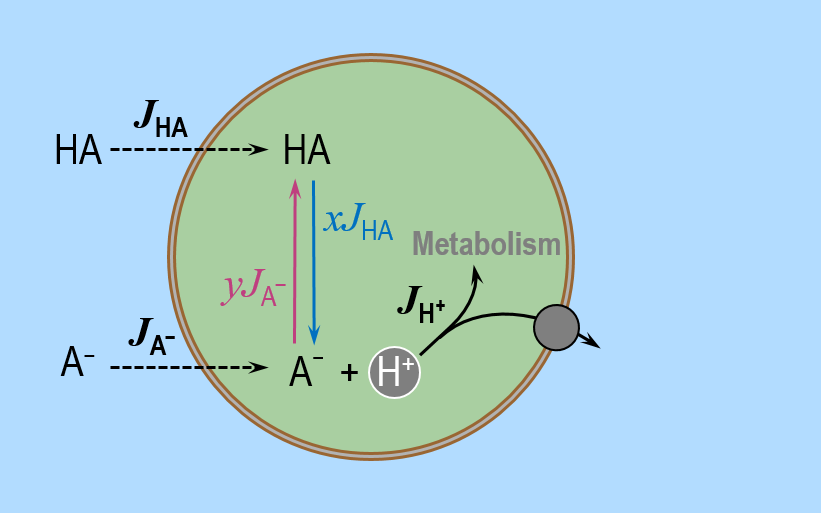
\includegraphics[width=0.5\linewidth]{img/Figure 3.png}
\caption{\label{fig:3} Cartoon illustrating the main assumptions in the BDW model of permeating uncharged weak acid $\mathrm{HA}$ and its conjugate anionic weak base $\mathrm{A^-}$. The BDW model consists of two time-dependent ODEs. The first one describes the time-course of the intracellular concentration of total weak acid $\mathrm{[TA]_i}$, and the second one describes the time-course of $\mathrm{[H^+]_i}$. BDW assumed that $\mathrm{[TA]_i}$ changes in time because of the transmembrane fluxes of $\mathrm{HA}$ ($J_\mathrm{HA}$) --- modelled according to Fick's first law of diffusion --- and $\mathrm{A^-}$ ($J_\mathrm{A^-}$) --- modelled according to the Goldman, Hodgkin, Katz (GHK) equation. According to BDW, the time rate of change of $\mathrm{[H^+]_i}$ depends on the net rate $\mathrm{d}Q/\mathrm{d}t$ at which acids are added into the cytosol. BDW assumed that $\mathrm{d}Q/\mathrm{d}t$ depends on (i) the release of $\mathrm{H^+}$ by some fraction $x$ of the entering $\mathrm{HA}$ (\emph{i.e.}, $xJ_\mathrm{HA}$), (ii) the consumption of $\mathrm{H^+}$ by some fraction $y$ of the entering $\mathrm{A^-}$ (\emph{i.e.}, $yJ_\mathrm{A^-}$), and (iii) the additional rate of intracellular $\mathrm{H^+}$ consumption via metabolism or active acid extrusion ($J_\mathrm{H^+}$).}
\end{figure}

Later, Bevensee and Boron defined the time rate of change per unit volume (\emph{e.g.}, $\mathrm{d[TA]_i/dt}$) as a `pseudoflux' $\phi$, with the area-to-volume ratio folded into the value of $\phi$ \citep{bevensee2013control}. Physiologists sometimes prefer to present experimental data in terms of pseudoflux because most mammalian cells often have complex geometries that make it difficult to estimate surface area.

In deriving the second ODE of their model, BDW started by noting that the time rate of change of free protons, $\mathrm{d[H^+]_i}/\mathrm{d}t$, depends on the rate at which acids are added into the cytosol per unit volume and per unit time --- denoted $\mathrm{d}Q/\mathrm{d}t$ ($\mathrm{mol\cdot m^{-3}\cdot s^{-1}}$) where $Q$ is the total intracellular acid content. Like $\mathrm{d[TA]_i}/\mathrm{d}t$, both $\mathrm{d[H^+]_i}/\mathrm{d}t$ and $\mathrm{d}Q/\mathrm{d}t$ are pseudofluxes.

In their simple system of a squid giant axon exposed to $\mathrm{CO_2}$ (\emph{i.e.}, $\mathrm{HA}$) and $\mathrm{HCO_3^-}$ (\emph{i.e.}, $\mathrm{A^-}$), BDW assumed that only three general processes affect $\mathrm{d}Q/\mathrm{d}t$: (i) the release of $\mathrm{H^+}$ by some fraction ($x$) of the entering $\mathrm{HA}$ (\emph{i.e.}, $xJ_\mathrm{HA}$), (ii) the consumption of $\mathrm{H^+}$ by some fraction $(y)$ of the entering $\mathrm{A^-}$ (\emph{i.e.}, $yJ_\mathrm{A^-}$), and (iii) the ``additional'' rate of intracellular consumption or active extrusion of $\mathrm{H^+}$ ($J_\mathrm{H^+}$; see \autoref{fig:3}) above the fixed background rate of $\mathrm{H^+}$ extrusion necessary to balance the fixed background rate of acid loading (\emph{i.e.}, addition of $\mathrm{H^+}$ or equivalent acid, or removal of $\mathrm{OH^-}$ or equivalent base) in the absence of $\mathrm{HA}/\mathrm{A^-}$. Thus,
\begin{equation}
\dfrac{\mathrm{d}Q}{\mathrm{d}t}=\rho\left(xJ_\mathrm{HA}-yJ_\mathrm{A^-}-J_\mathrm{H^+}\right).
\label{eqn:rate_Q}
\end{equation}
A critical insight by BDW is that during each infinitesimal increment in time during which a bolus of $\mathrm{HA}$ enters the cell, the entering $\mathrm{HA}$ redistributes itself between $\mathrm{HA}$ (and $\mathrm{H^+}$) vs $\mathrm{A^-}$, according to the pre-existing ratios $\mathrm{[HA]_i}/\mathrm{[TA]_i}$ and $\mathrm{[A^-]_i}/\mathrm{[TA]_i}$. Thus, the fraction $y$ of entering $\mathrm{HA}$ that remains $\mathrm{HA}$ is
\begin{equation}
y=\dfrac{\mathrm{[HA]_i}}{\mathrm{[TA]_i}}=\dfrac{\mathrm{[HA]_i}}{\mathrm{[HA]_i}+\mathrm{[A^-]_i}}.
\end{equation}
This is also the fraction of entering $\mathrm{A^-}$ that combines with $\mathrm{H^+}$ and becomes $\mathrm{HA}$. Combining the above expression with \autoref{eqn:K_A},
\begin{equation}
y=\dfrac{\mathrm{[HA]_i}}{\mathrm{[HA]_i}+\mathrm{[A^-]_i}}=\dfrac{\mathrm{[H^+]_i}}{\mathrm{[H^+]_i}+K_\mathrm{HA}}=\alpha,
\label{eqn:y}
\end{equation}
which BDW defined as $\alpha$. Conversely, the fraction $x$ of $\mathrm{A^-}$ that remains $\mathrm{A^-}$ is
\begin{equation}
x=\dfrac{\mathrm{[A^-]_i}}{\mathrm{[HA]_i}+\mathrm{[A^-]_i}}.
\end{equation}
This is also the fraction of entering $\mathrm{HA}$ that dissociates to form $\mathrm{A^-}$ and $\mathrm{H^+}$. Combining the above expression with \autoref{eqn:K_A},
\begin{equation}
x=\dfrac{\mathrm{[A^-]_i}}{\mathrm{[HA]_i}+\mathrm{[A^-]_i}}=\dfrac{K_\mathrm{HA}}{\mathrm{[H^+]_i}+K_\mathrm{HA}}=1-\alpha.
\label{eqn:y2}
\end{equation}
In summary, \autoref{eqn:rate_Q} becomes:
\begin{equation}
\dfrac{\mathrm{d}Q}{\mathrm{d}t}=\rho\bigg((1-\alpha)J_\mathrm{HA}-\alpha J_\mathrm{A^-}-J_\mathrm{H^+}\bigg).
\label{eqn:Q_rate2}
\end{equation}
BDW modelled $J_\mathrm{H^+}$ ($\mathrm{mol\cdot m^{-2}\cdot s^{-1}}$) as the additional proton-extrusion rate above the fixed background rate 
\begin{equation}
J_\mathrm{H^+}= 
\begin{cases}
  \dfrac{k}{\rho}\bigg(\mathrm{[H^+]_i}-\mathrm{[H^+]'_i}\bigg)  & \mathrm{pH_i} < \mathrm{{pH}'_i}, \\
  0  & \mathrm{otherwise},
\end{cases}
\label{eqn:pump}
\end{equation}
where $k$ ($\mathrm{s^{-1}}$) is the proton-pumping rate constant, $(k/\rho)\mathrm{[H^+]_i}$ is the additional flux of $\mathrm{H^+}$ above the background $\mathrm{H^+}$ flux of $(k/\rho)\mathrm{[H^+]'_i}$, which occurs at the resting $\mathrm{[H^+]_i}$ of $\mathrm{[H^+]'_i}$ (\emph{i.e.}, resting $\mathrm{pH_i}$ of $\mathrm{{pH}'_i}$). Note that $k/\rho$ has units of ($\mathrm{m\cdot s^{-1}}$), consistent with the membrane permeability terms $P_\mathrm{HA}$ and $P_\mathrm{A^-}$ in \autoref{eqn:J_HA} and \autoref{eqn:J_A}.\footnote{In the BDW paper, the final equation before the Appendix had a typographical error, omitting the $\rho$ in the following equation: $M_\mathrm{H} = (k/\rho)(\mathrm{[H^+]}-\mathrm{[H^+]}')$, where $M_\mathrm{H}$ is a flux (today represented as $J_\mathrm{H}$). Indeed, WFB had included $\rho$ in his extant Fortran code.}

The BDW authors used the definition of buffering power, in its infinitesimal form, to derive the relation between $\mathrm{d}{\mathrm{[H^+]_i}}/\mathrm{d}t$ and $\mathrm{d}Q/\mathrm{d}t$, as shown in the following steps.

Our first goal is to obtain an expression for $\mathrm{d}{\mathrm{pH}}/\mathrm{d}t$ in terms of $\mathrm{d}Q/\mathrm{d}t$. According to the chain rule:
\begin{equation}
\dfrac{\mathrm{dpH}}{\mathrm{d}t}=\left(\dfrac{\mathrm{dpH}}{\mathrm{d}Q}\right) \left(\dfrac{\mathrm{d}Q}{\mathrm{d}t}\right).
\label{eqn:pH_chain}
\end{equation}
By definition (see \autoref{eqn:buffer}), $\beta=-{\mathrm{d}Q}/{\mathrm{dpH}}$ ($\mathrm{mol\cdot m^{-3}}$), or equivalently
\begin{equation}
\dfrac{\mathrm{dpH}}{\mathrm{d}Q}=-\dfrac{1}{\beta}.
\label{eqn:pH_rate}
\end{equation}
Combining \autoref{eqn:pH_chain} and \autoref{eqn:pH_rate}
\begin{equation}
\dfrac{\mathrm{dpH}}{\mathrm{d}t}=\left(-\dfrac{1}{\beta}\right)\left(\dfrac{\mathrm{d}Q}{\mathrm{d}t}\right).
\label{eqn:pH_rate2}
\end{equation}
Our next goal is to obtain an expression for $\dfrac{\mathrm{dpH}}{\mathrm{d}t}$ in terms of $\dfrac{\mathrm{d[H^+]_i}}{\mathrm{d}t}$. According to the chain rule:
\begin{equation}
\dfrac{\mathrm{dpH}}{\mathrm{d}t}=\left(\dfrac{\mathrm{dpH}}{\mathrm{d[H^+]_i}}\right)\left( \dfrac{\mathrm{d[H^+]_i}}{\mathrm{d}t}\right).
\label{eqn:pH_rate3}
\end{equation}
By definition, $\mathrm{pH}={-\ln{\mathrm{[H^+]_i}}}/{2.303}$, so that:
\begin{equation}
\dfrac{\mathrm{dpH}}{\mathrm{d}{\mathrm{[H^+]_i}}}=-\dfrac{1}{2.303\mathrm{[H^+]_i}}.
\label{eqn:pH_rate4}
\end{equation}
Combining \autoref{eqn:pH_rate3} and \autoref{eqn:pH_rate4}, we have
\begin{equation}
\dfrac{\mathrm{dpH}}{\mathrm{d}t}=\left(-\dfrac{1}{2.303\mathrm{[H^+]_i}}\right)\left(\dfrac{\mathrm{d}\mathrm{[H^+]_i}}{\mathrm{d}t}\right),
\end{equation}
or equivalently,
\begin{equation}
\dfrac{\mathrm{d[H^+]_i}}{\mathrm{dt}}=-2.303\mathrm{[H^+]_i}\left(\dfrac{\mathrm{dpH}}{\mathrm{d}t}\right).
\label{eqn:H_rate}
\end{equation}
Substituting \autoref{eqn:pH_rate2} into \autoref{eqn:H_rate}, we obtain
\begin{equation}
\dfrac{\mathrm{d[H^+]_i}}{\mathrm{dt}}=\left(\dfrac{2.303\mathrm{[H^+]_i}}{\beta}\right)\left(\dfrac{\mathrm{d}Q}{\mathrm{d}t}\right).
\label{eqn:H_rate2}
\end{equation}
Finally, substituting \autoref{eqn:Q_rate2} into \autoref{eqn:H_rate2},
\begin{equation}
\dfrac{\mathrm{d[H^+]_i}}{\mathrm{dt}}=\left(\dfrac{2.303\mathrm{[H^+]_i}}{\beta}\right) \rho\bigg((1-\alpha)J_\mathrm{HA}-\alpha J_\mathrm{A^-}-J_\mathrm{H^+}\bigg),
\label{eqn:H_rate3}
\end{equation}
which is the second equation of the BDW model.

Substituting for $\alpha$ (from \autoref{eqn:y}), $[\mathrm{HA]_i} = \alpha [\mathrm{TA]_i}, [\mathrm{A^-]_i} = (1-\alpha) [\mathrm{TA]_i}$, in \autoref{eqn:TArate} and \autoref{eqn:H_rate3}, we obtain the two ODEs of the BDW model in terms of $[\mathrm{TA]_i}$ and $\mathrm{[H^+]_i}$:
\begin{equation}
\dfrac{\mathrm{d[TA]_i}}{\mathrm{d}t}=\rho\left(J_\mathrm{HA}+J_\mathrm{A^-}\right),
\label{eqn:TA_rate_final}
\end{equation}
\begin{equation}
\dfrac{\mathrm{d[H^+]_i}}{\mathrm{d}t}=\left(\dfrac{2.303\mathrm{[H^+]_i}}{\beta}\right)\rho\left(\left(\dfrac{K_\mathrm{HA}}{\mathrm{[H^+]_i}+K_\mathrm{HA}}\right)J_\mathrm{HA}-\left(\dfrac{\mathrm{[H^+]_i}}{\mathrm{[H^+]_i}+K_\mathrm{HA}}\right)J_\mathrm{A^-}-J_\mathrm{H^+} \right),
\label{eqn:H_rate_final}
\end{equation}
where $J_\mathrm{HA}$ (from \autoref{eqn:J_HA}), and $J_\mathrm{A^-}$ (from \autoref{eqn:J_A}) are given by:
\begin{equation*}
J_\mathrm{HA}=P_\mathrm{HA}\left( \mathrm{[HA]_o}-\dfrac{\mathrm{[H^+]_i}}{\mathrm{[H^+]_i}+K_\mathrm{{HA}}}\mathrm{[TA]_i} \right),
\end{equation*}
\begin{equation*}
J_\mathrm{A^-}=P_\mathrm{A^-}\left(\dfrac{V_\mathrm{m}F}{RT}\right)\left(\dfrac{\mathrm{[A^-]_o}-\dfrac{K_\mathrm{HA}}{\mathrm{[H^+]_i}+K_\mathrm{HA}}\mathrm{[TA]_i} \epsilon}{1-\epsilon}\right),
\end{equation*}
and $J_\mathrm{H^+}$ is given by \autoref{eqn:pump}.

The numerical solution of the above two equations yields the time courses of $[\mathrm{TA]_i}$ and $\mathrm{[H^+]_i}$, which in turn yield the time-courses of $[\mathrm{HA]_i}$ and $[\mathrm{A^-]_i}$ via:
\begin{equation}
\mathrm{[HA]_i}=\alpha\mathrm{[TA]_i},
\end{equation}
\begin{equation}
\mathrm{[A^-]_i}=(1-\alpha)\mathrm{[TA]_i},
\end{equation}
where
\begin{equation}
\alpha=\dfrac{\mathrm{[H^+]_i}}{\mathrm{[H^+]_i}+K_\mathrm{HA}}.
\label{eqn:alpha}
\end{equation}

\paragraph{Simulation for $\mathrm{CO_2}/\mathrm{HCO_3^-}$ experiments.}

BDW employed \autoref{eqn:TA_rate_final} and \autoref{eqn:H_rate_final} to simulate the experiments in which they exposed a squid giant axon to a solution containing equilibrated $\mathrm{CO_2}/\mathrm{HCO_3^-}$. Their simulation protocol was a step change in (a) extracellular $p_\mathrm{CO_2}$ from $0$ to $5\%$ $\mathrm{CO_2}$ ($37$ $\mathrm{mmHg}$ or, with $s=0.0321$ $\mathrm{mM\cdot mmHg^{-1}}$, $\mathrm{[CO_2]_o}=s.p_\mathrm{CO_2}=1.1877~\mathrm{mM}$) and (b) extracellular $\mathrm{[HCO_3^-]}$ from $0$ to $59.5260$ $\mathrm{mM}$ (the value that $\mathrm{[HCO_3^-]_o}$ has in a solution containing $5\%$ $\mathrm{CO_2}$ at $\mathrm{pH_o}$ of $7.70$)\footnote{BDW arrived at the value $\mathrm{[HCO_3^-]_o}= 59.5260$ $\mathrm{mM}$ by rearranging the equilibrium relation for $\mathrm{CO_2}/\mathrm{HCO_3^-}$ outside the cell: $\mathrm{[HCO_3^-]_o}=\dfrac{K_\mathrm{CO_2}\mathrm{[CO_2]_o}}{\mathrm{[H^+]_o}}= 59.5260$ $\mathrm{mM}$, when $K_\mathrm{CO_2}= 1\times 10^{-3}$ $\mathrm{mM}$ (or equivalently, $\mathrm{pK_{CO_2}}=-\log(K_\mathrm{CO_2})=6.0$), $\mathrm{[CO_2]_o}= 1.1877$ and $\mathrm{pH_o}= 7.70$.}. The step change is applied for $2700$ $\mathrm{s}$ ($45~\mathrm{min}$) at constant $\mathrm{pH_o}=7.70$.

\autoref{table1} and \autoref{table2} report the parameter values used by BDW. \autoref{table1} provides parameter values that are common to both the $\mathrm{CO_2}/\mathrm{HCO_3^-}$ and the $\mathrm{NH_3}/\mathrm{NH_4^+}$ experiments. \autoref{table2} provides parameter values exclusive to the $\mathrm{CO_2}/\mathrm{HCO_3^-}$ experiments only.

\begin{table}[hbt!]
\caption{Parameter values used in both simulations of squid-axon $\mathrm{CO_2}/\mathrm{HCO_3^-}$ experiments and $\mathrm{NH_3}/\mathrm{NH_4^+}$ experiments.}\label{table1}
\begin{threeparttable}
\def\arraystretch{1.5}
\begin{tabular}{c|c|c|c|c|c}
\toprule
Symbol & Name & BDW Value & Unit & New Value & Unit \\ 
\midrule
$\mathrm{T}$ & temperature & $23$ ($296.15$) & \textdegree $\mathrm{C}$ (\textdegree $\mathrm{K}$) & & \\ 
$\mathrm{R}$ & gas constant & $8.314$ & $\mathrm{J\cdot mol^{-1}\cdot K^{-1}}$ & & \\ 
$\mathrm{F}$ & Faraday constant & $96485$ & $\mathrm{C\cdot mol^{-1}}$ & & \\ 
$\rho$ & area/volume ratio & $0.008$\tnote{1} &  $\mu\mathrm{m}^{-1}$  & $8000$ &  $\mathrm{m}^{-1}$ \\
$\mathrm{pH_o}$ & extracellular $\mathrm{pH}$ & $7.70$ & & &  \\ 
\bottomrule
\end{tabular}
\begin{tablenotes}
\item[1] Note that BDW did not report the value of $\rho$, but rather the value of the fiber (\emph{i.e.}, axon) diameter, which is equal to $500$ $\mu\mathrm{m}$ and corresponds to a $\rho$ of $0.008$ $\mu\mathrm{m}^{-1}$ or $8000$ $\mathrm{m}^{-1}$.
\end{tablenotes}
\end{threeparttable}
\end{table}

\begin{table}[hbt!]
\caption{Parameter values for simulations of squid-axon $\mathrm{CO_2}/\mathrm{HCO_3^-}$ experiments.}\label{table2}
\begin{threeparttable}
\def\arraystretch{1.5}
\begin{tabular}{c|c|c|c|c|c}
\toprule
Symbol & Name & BDW Value & Unit & New Value & Unit \\ 
\midrule
$\beta_\mathrm{CO_2}$ & buffering power & $-26$ & $\mathrm{mM}$ & $26$ & $\mathrm{mM}$ \\ 
$s$ & solubility constant for $\mathrm{CO_2}$ & $0.0321$ \tnote{1} & $\mathrm{mM}/\mathrm{mmHg}$ & $0.241$ & $\mathrm{mM}/\mathrm{KPa}$ \\ 
$p_\mathrm{CO_2}$ & partial pressure of $\mathrm{CO_2}$ & $37$ & $\mathrm{mmHg}$ & $4.933$ & $\mathrm{KPa}$ \\ 
$p_\mathrm{CO_2}$ & partial pressure of $\mathrm{CO_2}$ & $37$ & $\mathrm{mmHg}$ & $4.933$ & $\mathrm{KPa}$ \\ 
${\mathrm{[CO_2]_o}}$ & extracellular $\mathrm{CO_2}$ & $1.1877$ & $\mathrm{mM}$ & & \\ 
${\mathrm{[HCO_3^-]_o}}$ & extracellular $\mathrm{HCO_3^-}$ & $59.5260$ & $\mathrm{mM}$ & & \\ 
$P_{\mathrm{CO_2}}$ & membrane permeability & $6\times 10^{-3}$ & $\mathrm{cm\cdot s^{-1}}$ & $6\times 10^{-5}$ & $\mathrm{m\cdot s^{-1}}$ \\ 
$P_{\mathrm{HCO_3^-}}$ & membrane permeability & $5\times 10^{-7}$ & $\mathrm{cm\cdot s^{-1}}$ & $5\times 10^{-9}$ & $\mathrm{m\cdot s^{-1}}$ \\
$K_\mathrm{CO_2}$ & acid dissociation constant & $10^{-3}$ & $\mathrm{mM}$ & & \\
$\mathrm{pK_{CO_2}}$ & acid dissociation constant & $6.0$ & & & \\
$V_\mathrm{m}$ & membrane potential & $-57$ \tnote{2} & $\mathrm{mV}$ & $-0.057$ & $\mathrm{V}$ \\
$k$ & $\mathrm{H^+}$ pump rate constant & $0-300$ \tnote{3} & $\mathrm{s^{-1}}$ & & \\
$\mathrm{pH_i}$ & intracellular $\mathrm{pH}$ & $7.40$ & & & \\
$\mathrm{{pH}'_i}$ & basal $\mathrm{pH}$ & $7.30$ \tnote{4} & & & \\ 
\bottomrule
\end{tabular}
\begin{tablenotes}
\item[1] Note that BDW did not report the value of $s$. This value is inferred from a $p_\mathrm{CO_2}$ of $37$ $\mathrm{mmHg}$ (reported in the legend of BDW's figure 6) and a $\mathrm{[CO_2]_o}$ of $1.1877$ $\mathrm{mM}$ (in the original Fortran code). Although BDW reported a value for $s$ of $0.0346$ $\mathrm{mM}/\mathrm{mmHg}$ (taken from \cite{harned1943ionization}, referring to $0.5~\mathrm{M}$ $\mathrm{NaCl}$ at $20$\textdegree $\mathrm{C}$), they used this value only for the Davenport diagram in their figure 5A.
\item[2] BDW did not report the value of $V_\mathrm{m}$, but in the Fortran code, used $-57~\mathrm{mV}$, which matched the measured mean value.
\item[3] In figure 6A of the BDW paper, the proton pumping rate constant ($k$) had values of $0$, $10$, $75$, $150$, or $300~\mathrm{s}^{-1}$.
\item[4] BDW did not report this value, but in their code used $7.30$.
\end{tablenotes}
\end{threeparttable}
\end{table}

In the present work, the differential \autoref{eqn:TA_rate_final} and \autoref{eqn:H_rate_final} --- when coded in CellML and solved with OpenCOR --- produce the plots in \autoref{fig:4}. The simulation file Boron-CO2.sedml contains the computational setting for running the model. Open the .sedml file in OpenCOR and click Run Simulation. The initial conditions are $[\mathrm{TA]_i}=0$ $\mathrm{mM}$ and $\mathrm{pH_i}=7.40$. Note that \autoref{fig:4} illustrates the time courses not only of $\mathrm{pH_i}$ --- as presented by BDW --- but also of quantities (\emph{e.g.}, various solute concentrations and fluxes) not displayed in the original paper; these values are useful for understanding the processes that contribute to the $\mathrm{pH_i}$ transient. Moreover, our curated and annotated version of the BDW model also allows one to alter the parameter values from those originally chosen by BDW, thereby extending the ability of the user to investigate the predictive power of the computational model.

\begin{figure}[ht!]
\centering
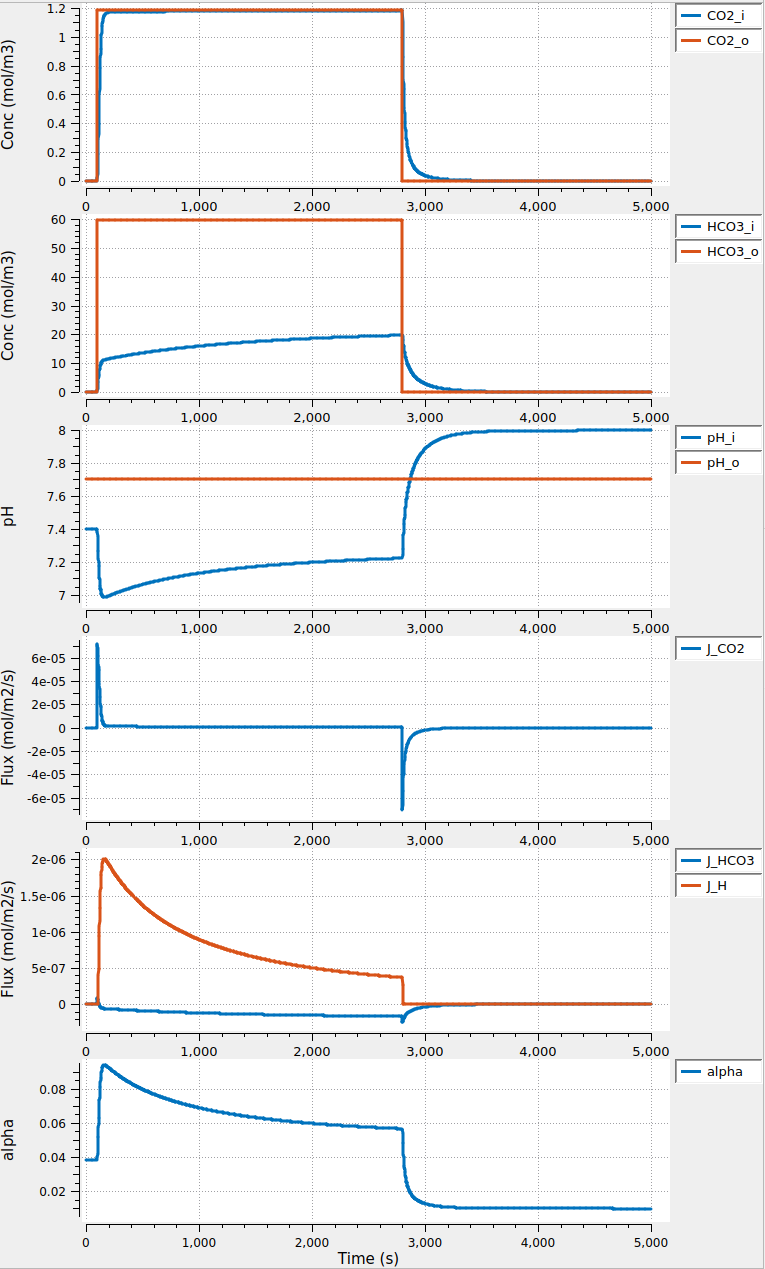
\includegraphics[width=0.8\linewidth]{img/Figure 4.png}
\caption{\label{fig:4} Solution of the BDW model during and following a $2700~\mathrm{s}$ period of externally applied $\mathrm{CO_2}$. In these simulations $\mathrm{pH_o}=7.70$ and $\mathrm{[HCO_3^-]_o}$ is determined from the equilibrium with $\mathrm{[H^+]_o}$ and $\mathrm{CO_2}$ (footnote 9). Note that, during the plateau phase, $\mathrm{[HCO_3^-]_i}$ continues to rise as $\mathrm{pH_i}$ rises at a constant $\mathrm{[CO_2]_i}$ (the proton pumping rate $k$ is set to $300$ $\mathrm{s^{-1}}$, thus $k/\rho= 0.0375$ $\mathrm{m\cdot s^{-1}}$). Note also that, after the removal of $\mathrm{CO_2}/\mathrm{HCO_3^-}$, $\mathrm{pH_i}$ rises to a higher value ($\sim 8.15$) than its starting value ($\sim 7.4$), indicating the net extrusion of acid from the cell during the $\mathrm{CO_2}/\mathrm{HCO_3^-}$ exposure.}
\end{figure}

\section{The Boron \& De Weer Model for the Permeation by an Uncharged Weak Base and its Conjugate, Cationic Weak Acid}

Following an approach analogous to the one outlined above for weak acids, BDW derived two time-dependent ODEs. The first describes the time-course of the concentration of total intracellular buffer ($[\mathrm{TB]_i} = [\mathrm{B]_i}+[\mathrm{BH^+]_i}$), and the other the time-course of the intracellular free $\mathrm{[H^+]_i}$, for any buffer pair $\mathrm{B}/\mathrm{BH^+}$.

\paragraph{Derivation for weak bases.}

Imagine that a cell is exposed to a solution containing equilibrated $\mathrm{B}/\mathrm{BH^+}$, and that both $\mathrm{B}$ and $\mathrm{BH^+}$ initially move into the cell --- because of the chemical gradient in the case of $\mathrm{B}$, and because of the electrochemical gradient in the case of $\mathrm{BH^+}$.

\begin{figure}[ht]
\centering
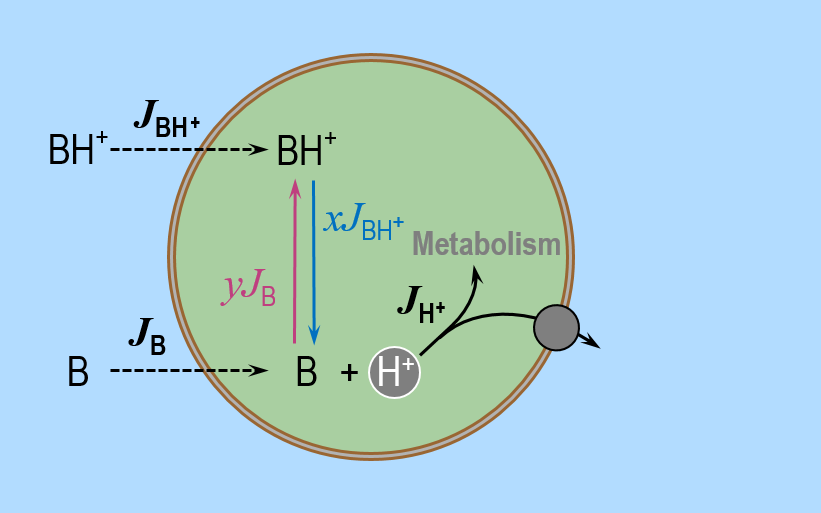
\includegraphics[width=0.5\linewidth]{img/Figure 5.png}
\caption{\label{fig:5} Cartoon illustrating the main assumptions in the BDW model of permeating uncharged weak base $\mathrm{B}$ and its conjugate anionic weak acid $\mathrm{BH^+}$. The BDW model consists of two time-dependent ODEs. The first one describes the time-course of the intracellular concentration of total weak base $\mathrm{[TB]_i}$, and the second one describes the time-course of $\mathrm{[H^+]_i}$. BDW assumed that $\mathrm{[TB]_i}$ changes in time because of the transmembrane fluxes of $\mathrm{HA}$ ($J_\mathrm{B}$) --- modelled according to Fick's first law of diffusion --- and $\mathrm{BH^+}$ ($J_\mathrm{BH^+}$) --- modelled according to the Goldman, Hodgkin, Katz (GHK) equation. According to BDW, the time rate of change of $\mathrm{[H^+]_i}$ depends on the net rate $\mathrm{d}Q/\mathrm{d}t$ at which acids are added into the cytosol. BDW assumed that $\mathrm{d}Q/\mathrm{d}t$ depends on (i) the release of $\mathrm{H^+}$ by some fraction $x$ of the entering $\mathrm{BH^+}$ (\emph{i.e.}, $xJ_\mathrm{BH^+}$), (ii) the consumption of $\mathrm{H^+}$ by some fraction $y$ of the entering $\mathrm{B}$ (\emph{i.e.}, $yJ_\mathrm{B}$), and (iii) the additional rate of intracellular $\mathrm{H^+}$ consumption via metabolism or active acid extrusion ($J_\mathrm{H^+}$).}
\end{figure}

Assuming, as in \autoref{fig:5}, that $\mathrm{[TB]_i}$ only can change due to the transmembrane fluxes of $\mathrm{B}$ ($J_\mathrm{B}$) and $\mathrm{BH^+}$ ($J_{\mathrm{BH^+}}$), the time rate of change of $\mathrm{[TB]_i]}$ --- analogous to \autoref{eqn:TArate} above --- is
\begin{equation}
\dfrac{\mathrm{d[TB]_i}}{\mathrm{d}t}=\rho\left(J_\mathrm{B}+J_\mathrm{BH^+}\right),
\label{eqn:TB_rate}
\end{equation}
where $\rho$ ($\mathrm{m^{-1}}$) is again the area-to-volume ratio for the cell. The equation
\begin{equation}
J_\mathrm{B}=P_\mathrm{B}\bigg(\mathrm{[B]_o}-\mathrm{[B]_i}\bigg),
\label{eqn:J_B}
\end{equation}
is an integrated form of Fick's first law of diffusion that describes the net passive flux of B, and
\begin{equation}
J_\mathrm{BH^+}=P_\mathrm{BH^+}\left(\dfrac{V_\mathrm{m}F}{RT}\right)\left(\dfrac{\mathrm{[BH^+]_o}-\epsilon '\mathrm{[BH^+]_i}}{\epsilon '-1}\right),
\label{eqn:J_BH}
\end{equation}
describes the net passive influx of $\mathrm{BH^+}$ according to the GHK equation. In the previous two equations, $P_\mathrm{B}$ ($\mathrm{m\cdot s^{-1}}$) is the membrane permeability to the uncharged weak base $\mathrm{B}$, $P_\mathrm{{BH^+}}$ ($\mathrm{m\cdot s^{-1}}$) is the membrane permeability to the charged conjugate weak acid $\mathrm{BH^+}$, and $\epsilon '$ is a shorthand for $e^{{V_\mathrm{m}F}/{RT}}$. \autoref{eqn:TB_rate} is the first of two ODEs of the BDW model for the buffer pair $\mathrm{B}/\mathrm{BH^+}$.

The second equation of the BDW model for a weak base --- analogous to \autoref{eqn:H_rate3} above --- is
\begin{equation}
\dfrac{\mathrm{d[H^+]_i}}{\mathrm{d}t}=\left(\dfrac{2.303\mathrm{[H^+]_i}}{\beta}\right) \rho\bigg((1-\alpha)J_\mathrm{BH^+}-\alpha J_\mathrm{B}-J_\mathrm{H^+}\bigg),
\label{eqn:H_rate_B}
\end{equation}
where $J_\mathrm{H+}$ is the same as in \autoref{eqn:pump} and 
\begin{equation}
\alpha=\dfrac{\mathrm{[BH^+]_i}}{\mathrm{[BH^+]_i}+\mathrm{[B]_i}}=\dfrac{\mathrm{[H^+]_i}}{\mathrm{[H^+]_i}+K_\mathrm{BH^+}},
\label{eqn:alpha_B}
\end{equation}
and
\begin{equation}
1-\alpha=\dfrac{\mathrm{[B]_i}}{\mathrm{[BH^+]_i}+\mathrm{[B]_i}}=\dfrac{K_\mathrm{BH^+}}{\mathrm{[H^+]_i}+K_\mathrm{BH^+}}.
\label{eqn:alpha_B2}
\end{equation}
Substituting for $\alpha$, $[\mathrm{BH^+]_i} = \alpha [\mathrm{TB]_i}, [\mathrm{B]_i} = (1-\alpha) [\mathrm{TB]_i}$, $J_\mathrm{BH^+}$ , $J_\mathrm{B}$ in \autoref{eqn:TB_rate} and \autoref{eqn:H_rate_B}, we obtain the two ODEs of the BDW model in terms of $[\mathrm{TB]_i}$ and $\mathrm{[H^+]_i}$ 
\begin{equation}
\dfrac{\mathrm{d[TB]_i}}{\mathrm{d}t}=\rho\left(J_\mathrm{B}+J_\mathrm{BH^+} \right),
\label{eqn:TB}
\end{equation}
\begin{equation}
\dfrac{\mathrm{d[H^+]_i}}{\mathrm{d}t}=\dfrac{2.303\mathrm{[H^+]_i}}{\beta}\rho\left(\left(\dfrac{K_\mathrm{BH^+}}{\mathrm{[H^+]_i}+K_\mathrm{BH^+}}\right)J_\mathrm{BH^+}-\left(\dfrac{\mathrm{[H^+]_i}}{\mathrm{[H^+]_i}+K_\mathrm{BH^+}}\right)J_\mathrm{B}-J_\mathrm{H^+} \right),
\label{eqn:B_H}
\end{equation}
where
\begin{equation*}
J_\mathrm{BH^+}=P_\mathrm{BH^+}\left(\dfrac{V_\mathrm{m}F}{RT}\right)\left(\dfrac{\mathrm{[BH^+]_o}-\dfrac{\mathrm{[H^+]_i}}{\mathrm{[H^+]_i}+K_\mathrm{BH^+}}\mathrm{[TB]_i} \epsilon '}{\epsilon '-1}\right),
\end{equation*}
\begin{equation*}
J_\mathrm{B}=P_\mathrm{B}\left( \mathrm{[B]_o}-\dfrac{K_\mathrm{BH^+}}{\mathrm{[H^+]_i}+K_\mathrm{BH^+}}\mathrm{[TB]_i} \right),
\end{equation*}
and $J_\mathrm{H^+}$ is given by \autoref{eqn:pump}.

Numerically integrating the above two equations yields the time courses of $[\mathrm{TB]_i}$ and $\mathrm{[H^+]_i}$, from which we can compute the time-courses of $[\mathrm{BH^+]_i}$ and $[\mathrm{B]_i}$ from
\begin{equation}
\mathrm{[BH^+]_i}=\alpha\mathrm{[TB]_i},
\end{equation}
\begin{equation}
\mathrm{[B]_i}=(1-\alpha)\mathrm{[TB]_i},
\end{equation}
where
\begin{equation}
\alpha=\dfrac{\mathrm{[H^+]_i}}{\mathrm{[H^+]_i}+K_\mathrm{BH^+}}.
\end{equation}

\paragraph{Simulation for $\mathrm{NH_3}/\mathrm{NH_4^+}$ experiments.}

BDW employed \autoref{eqn:TB} and \autoref{eqn:B_H} to simulate the experiments in which they exposed a squid giant axon to equilibrated $\mathrm{NH_3}/\mathrm{NH_4^+}$. Their simulation protocol was a step change in extracellular $\mathrm{NH_4Cl}$ from $0$ to $9$ $\mathrm{mM}$ (that is, a step change in $\mathrm{[NH_4^+]_o}$ from $0$ to $8.86$ $\mathrm{mM}$, and in $\mathrm{[NH_3]_i}$ from $0$ to $0.14$ $\mathrm{mM}$) applied for $1500~\mathrm{s}$ ($25~\mathrm{min}$) at constant $\mathrm{pH_o}=7.70$.\footnote{BDW arrived at the value $\mathrm{[NH_4^+]_o}= 8.86~\mathrm{mM}$ by rearranging the equilibrium relation outside the cell: $\mathrm{[NH_4^+]_o}=\mathrm{[H^+]_o}\dfrac{\mathrm{[TB]_o}}{\mathrm{[H^+]_o}+K_\mathrm{NH_4^+}}= 8.86~\mathrm{mM}$, when $\mathrm{[TB]_o}= 9~\mathrm{mM}$, $\mathrm{pH_o}= 7.70$, and $K_\mathrm{NH_4^+} = 3.16\times 10^{-7}~\mathrm{mM}$ (or equivalently, $\mathrm{pK} = 9.50$). The extracellular $\mathrm{NH_3}$ concentration can be obtained as $\mathrm{[NH_3]_o}=\mathrm{[TB]_o}-\mathrm{[NH_4^+]_o}= 9-8.86 = 0.14~\mathrm{mM}$}

\autoref{table1} and \autoref{table3} report the parameter values used by BDW. Note that in the $\mathrm{NH_3}/\mathrm{NH_4^+}$ simulations, $k$ is always zero, that is, $J_\mathrm{H^+}$ does not affect these processes.

\begin{table}[hbt!]
\caption{Parameter values for simulations of squid-axon $\mathrm{NH_3}/\mathrm{NH_4^+}$ experiments.}\label{table3}
\begin{threeparttable}
\def\arraystretch{1.5}
\begin{tabular}{c|c|c|c|c|c}
\toprule
Symbol & Name & BDW Value & Unit & New Value & Unit \\ 
\midrule
$\beta_\mathrm{NH_4^+}$ & buffering power & $-9$ & $\mathrm{mM}$ & $9$ & $\mathrm{mM}$ \\ 
${\mathrm{[TB]_o}}$ & extracellular total ammonia & $9$ \tnote{1} & $\mathrm{mM}$ & & \\ 
${\mathrm{[NH_3]_o}}$ & extracellular $\mathrm{NH_3}$ & $0.1404$ & $\mathrm{mM}$ & & \\ 
${\mathrm{[NH_4^+]_o}}$ & extracellular $\mathrm{NH_4^+}$ & $8.8596$ & $\mathrm{mM}$ & & \\ 
$P_{\mathrm{NH_3}}$ & membrane permeability & $6\times 10^{-3}$ & $\mathrm{cm\cdot s^{-1}}$ & $6\times 10^{-5}$ & $\mathrm{m\cdot s^{-1}}$ \\ 
$P_{\mathrm{NH_4^+}}$ & membrane permeability & $0-1\times 10^{-4}$ \tnote{2} & $\mathrm{cm\cdot s^{-1}}$ & $1\times 10^{-6}$ & $\mathrm{m\cdot s^{-1}}$ \\
$K_\mathrm{NH_4^+}$ & acid dissociation constant & $0.31623\times10^{-6}$ & $\mathrm{mM}$ & & \\
$\mathrm{pK_{NH_4^+}}$ & acid dissociation constant & $9.5$ & & & \\
$V_\mathrm{m}$ & membrane potential & $-55$ \tnote{3} & $\mathrm{mV}$ & $-0.055$ & $\mathrm{V}$ \\ 
$k$ & $\mathrm{H^+}$ pump rate constant & $0$ & $\mathrm{s^{-1}}$ & & \\
$\mathrm{pH_i}$ & intracellular $\mathrm{pH}$ & $7.32$ \tnote{4} & & & \\
\bottomrule
\end{tabular}
\begin{tablenotes}
\item[1] In their original Fortran code that generated the plots in their figure 6B, BDW used $\mathrm{[TB]_o}=9~\mathrm{mM}$ (the value used in some of their early experiments), and not $10~\mathrm{mM}$ as (the value used in their later experiments) indicated in the figure and legend for figure 6B in their original paper.
\item[2] In figure 6B of the BDW paper, $P_\mathrm{NH_4^+}$ had values of $0$, $10^{-6}$, $10^{-5}$, and $10^{-4}$ $\mathrm{cm}^{-1}$.
\item[3] BDW did not report the value of $V_\mathrm{m}$, but in their code used $-55$ $\mathrm{mV}$, which matched the measured mean value.
\item[4] In their code BDW used the value of $7.32$ and not $7.30$, which they used when constructing the Davenport diagram in their figure 5B.
\end{tablenotes}
\end{threeparttable}
\end{table}

The differential \autoref{eqn:TB} and \autoref{eqn:B_H} --- when coded in CellML and solved with OpenCOR --- produce the plots in \autoref{fig:6}. The simulation file Boron-NH3.sedml contains the computational setting for running the model. Open the .sedml file in OpenCOR and click Run Simulation. The initial conditions are $[\mathrm{TB]_i} = 0$ $\mathrm{mM}$ and $\mathrm{pH_i}=7.32$.

\begin{figure}[ht!]
\centering
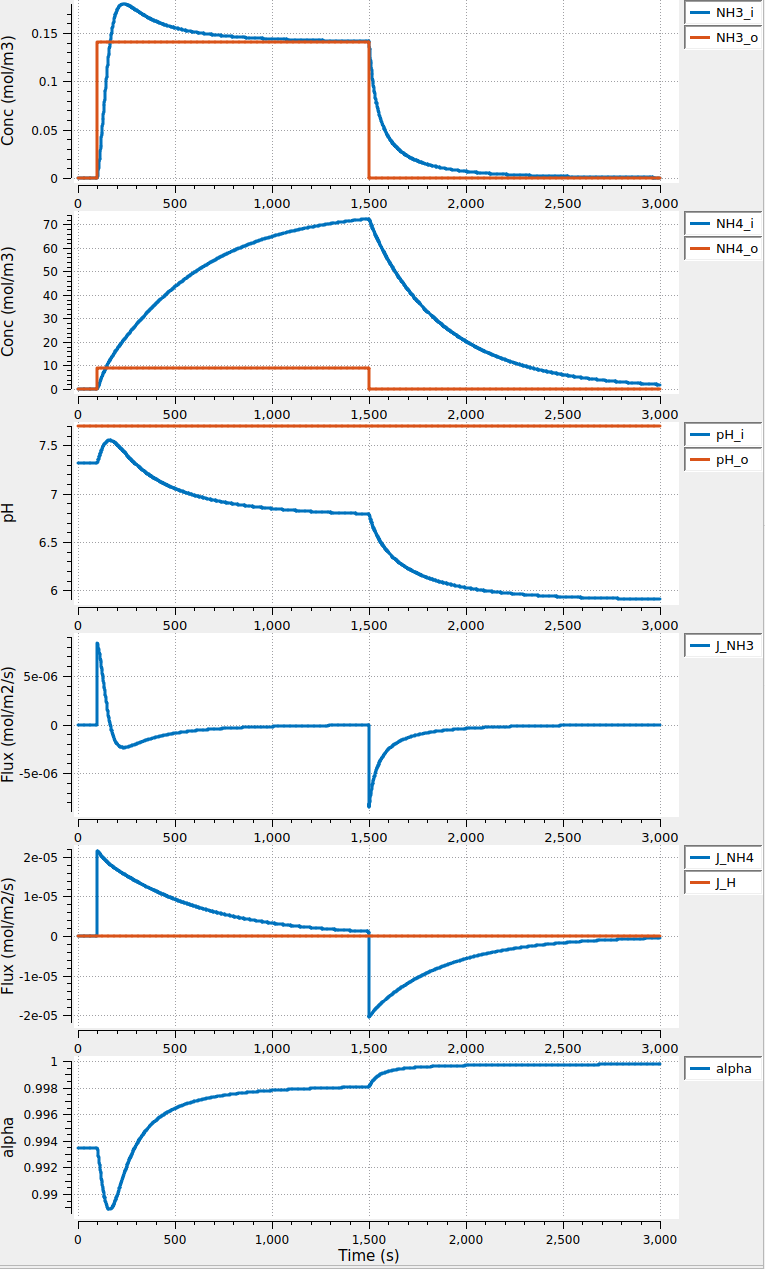
\includegraphics[width=0.8\linewidth]{img/Figure 6.png}
\caption{\label{fig:6} Solution of the BDW model during and following a $1500~\mathrm{s}$ period of externally applied $\mathrm{NH_4Cl}$. In these simulations $\mathrm{[NH_4^+]_o}=9$ $\mathrm{mM}$. The intracellular fluid becomes alkaline as $\mathrm{NH_3}$ enters (note the $J_\mathrm{NH_3}$ time course) and hydrates to form $\mathrm{NH_4^+}$ and $\mathrm{OH^-}$. Additional passive $\mathrm{NH_4^+}$ entry (note $J_\mathrm{NH_4^+}$ time course) down its electrochemical gradient opposes the effect of the $\mathrm{NH_3}$ entry and slightly reduces the $\mathrm{pH_i}$ increase. Upon removal of $\mathrm{NH_4Cl}$, $\mathrm{[NH_3]_i}$ and $\mathrm{[NH_4^+]_i}$ decay towards their original values, but $\mathrm{pH_i}$ drops well below its original value of $7.40$.}
\end{figure}

\section{Discussion}

The publication of this retrospective paper provides an opportunity to clarify some concepts in the original paper that have benefitted from subsequent experimental and theoretical advances. We also provide some additional parameters missing from BDW and correct some minor errors. Most importantly, the curated model is now freely available on the Physiome  website\footnote{\url{https://models.physiomeproject.org/workspace/5f8}} in standardised form (CellML) that can be run in the open source software OpenCOR. A follow-up paper will be written that recasts the equations in bond graph form to facilitate their incorporation into more complex models where $\mathrm{pH}$ regulation is coupled with other cellular processes.

\subsection{Historical Context}

The 1976 Boron \& De Weer paper introduced the first models to simulate the time course of $\mathrm{pH_i}$. By developing a predictive mathematical model based on first principles, BDW provided a quantitative basis for interpreting their new data on the time-dependent response of $\mathrm{pH_i}$ to step changes in extracellular $\mathrm{CO_2}/\mathrm{HCO_3^-}$ (and $\mathrm{HA}/\mathrm{A^-}$ pairs in general) and $\mathrm{NH_3}/\mathrm{NH_4^+}$ (and $\mathrm{B/BH^+}$ pairs in general). The models also provided a clear, quantitative basis for interpreting BDW's new data on how cells regulate their $\mathrm{pH_i}$, which BDW modelled as a $\mathrm{pH_i}$-dependent $\mathrm{H^+}$-extrusion mechanism. Below, we will introduce a broader concept termed ``acid extrusion'' \citep{boron1977intracellular}. The first of the two BDW models elucidates how the transmembrane fluxes of a neutral weak acid and its anionic conjugate weak base affects $\mathrm{pH_i}$, with the acid-extrusion becoming increasingly important as $\mathrm{pH_i}$ falls. The second model simulates how the transmembrane fluxes of a neutral base and its cationic conjugate weak acid affects $\mathrm{pH_i}$.

Of course, BDW were not the first to undertake a quantitative assessment of how acids or bases affect, or are affected by, the $\mathrm{pH}$ of a solution. Below, we divide the earlier work into two major categories, (a) analyses of how neutral weak acids (and their anion conjugate weak bases) or neutral weak bases (and their cationic conjugate weak acids) affect $\mathrm{pH}$ in simple systems, and (b) analyses of how the distribution of $\mathrm{HA}/\mathrm{A^-}$ (or $\mathrm{B}/\mathrm{BH^+}$) across a barrier, such as a cell membrane, are affected by $\mathrm{pH_i}$ and $V_\mathrm{m}$.

\subsection{Development of the Concept of Buffering in Simple and Complex Systems}

\paragraph{Buffering power.} 
In 1914, \cite{koppel1914wirkung} introduced the first modern definition of the chemical buffering (\emph{i.e.}, ``magnitude of moderation'', or $P$) of $\mathrm{H^+}$ by a weak-acid/weak-base conjugate pair, and --- based on first principles --- derived an expression for buffering power. Because these authors defined $P$ in terms of the amount of strong acid that one must add to a solution to produce a $\mathrm{pH}$ change, $P$ is a negative number. \cite{roos1980buffer} translated the Koppel-Spiro paper from its original German, and provided a historical context.

Initially unaware of the work of Koppel and Spiro, \cite{van1922measurement} independently defined buffering power --- to which he assigned the Greek letter $\beta$. Because he defined $\beta$ in terms of the amount of strong base that one must add to a solution to produce a $\mathrm{pH}$ change (see \autoref{eqn:buffer}), $\beta$ is a positive number. Although modest differences exist between the efforts of Koppel and Spiro on the one hand and Van Slyke on the other, they are quite similar. Nevertheless, it is Van Slyke's definition of $\beta$ that has become the modern convention throughout chemistry and physiological chemistry.

Koppel \& Spiro and Van Slyke quantitatively described how --- in a one-compartment solution --- weak acids, weak bases, ampholytes, and weak-acid/base mixtures can buffer added strong acid or strong base. In their analysis, the system both begins and ends in an equilibrium state. Of course, in their pioneering work, these authors had no reason to contemplate time courses or barriers separating more than one compartment.

In their work, BDW defined $\beta$ as a negative number, as Koppel and Spiro defined their $P$.

\paragraph{The ``Davenport'' diagram.} 
This nomogram \citep{boron2016medical} is a powerful tool for graphically computing the effects of respiratory acid-base disorders (caused by changes in $\mathrm{[CO_2]}$ in a system open to $\mathrm{CO_2}$) and metabolic acid-base disorders (caused by the addition or removal of $\mathrm{HCO_3^-}$ or a strong acid or base). The underlying assumption for the Davenport diagram is that the system is in equilibrium. The first component of a Davenport diagram (see \autoref{fig:7}) is a plot of $\mathrm{[HCO_3^-]}$ vs $\mathrm{pH_i}$ for one or more values of $\mathrm{[CO_2]}$ --- these are the $\mathrm{CO_2}$ isopleths that describe the equilibrium among $\mathrm{CO_2}$, $\mathrm{HCO_3^-}$, and $\mathrm{H^+}$. At any $\mathrm{pH}$ on any isopleth, the slope is the open-system $\mathrm{CO_2}/\mathrm{HCO_3^-}$ buffering power ($\beta_\mathrm{CO_2}$). The second component is a linear plot, on the same axes, of the concentration of all protonated forms of all non-$\mathrm{HCO_3^-}$ buffers vs $\mathrm{pH}$. At any $\mathrm{pH}$, the slope is the buffering power of all non-$\mathrm{HCO_3^-}$ buffers ($\beta_\mathrm{non-HCO_3^-}$), and the line is termed the non-$\mathrm{HCO_3^-}$ buffer line. Its linearity implies that $\beta_\mathrm{non-HCO_3^-}$ is insensitive to changes in $\mathrm{pH}$. The intersection of an isopleth with the non-$\mathrm{HCO_3^-}$ buffer line describes the current state of the system, when both $\mathrm{CO_2}/\mathrm{HCO_3^-}$ buffer and non-$\mathrm{HCO_3^-}$ buffers are simultaneously in equilibrium. Davenport developed a series of rules for using this paradigm to interpret acid-base disorders, and these rules are well founded in physical chemistry.

\begin{figure}[ht]
\centering
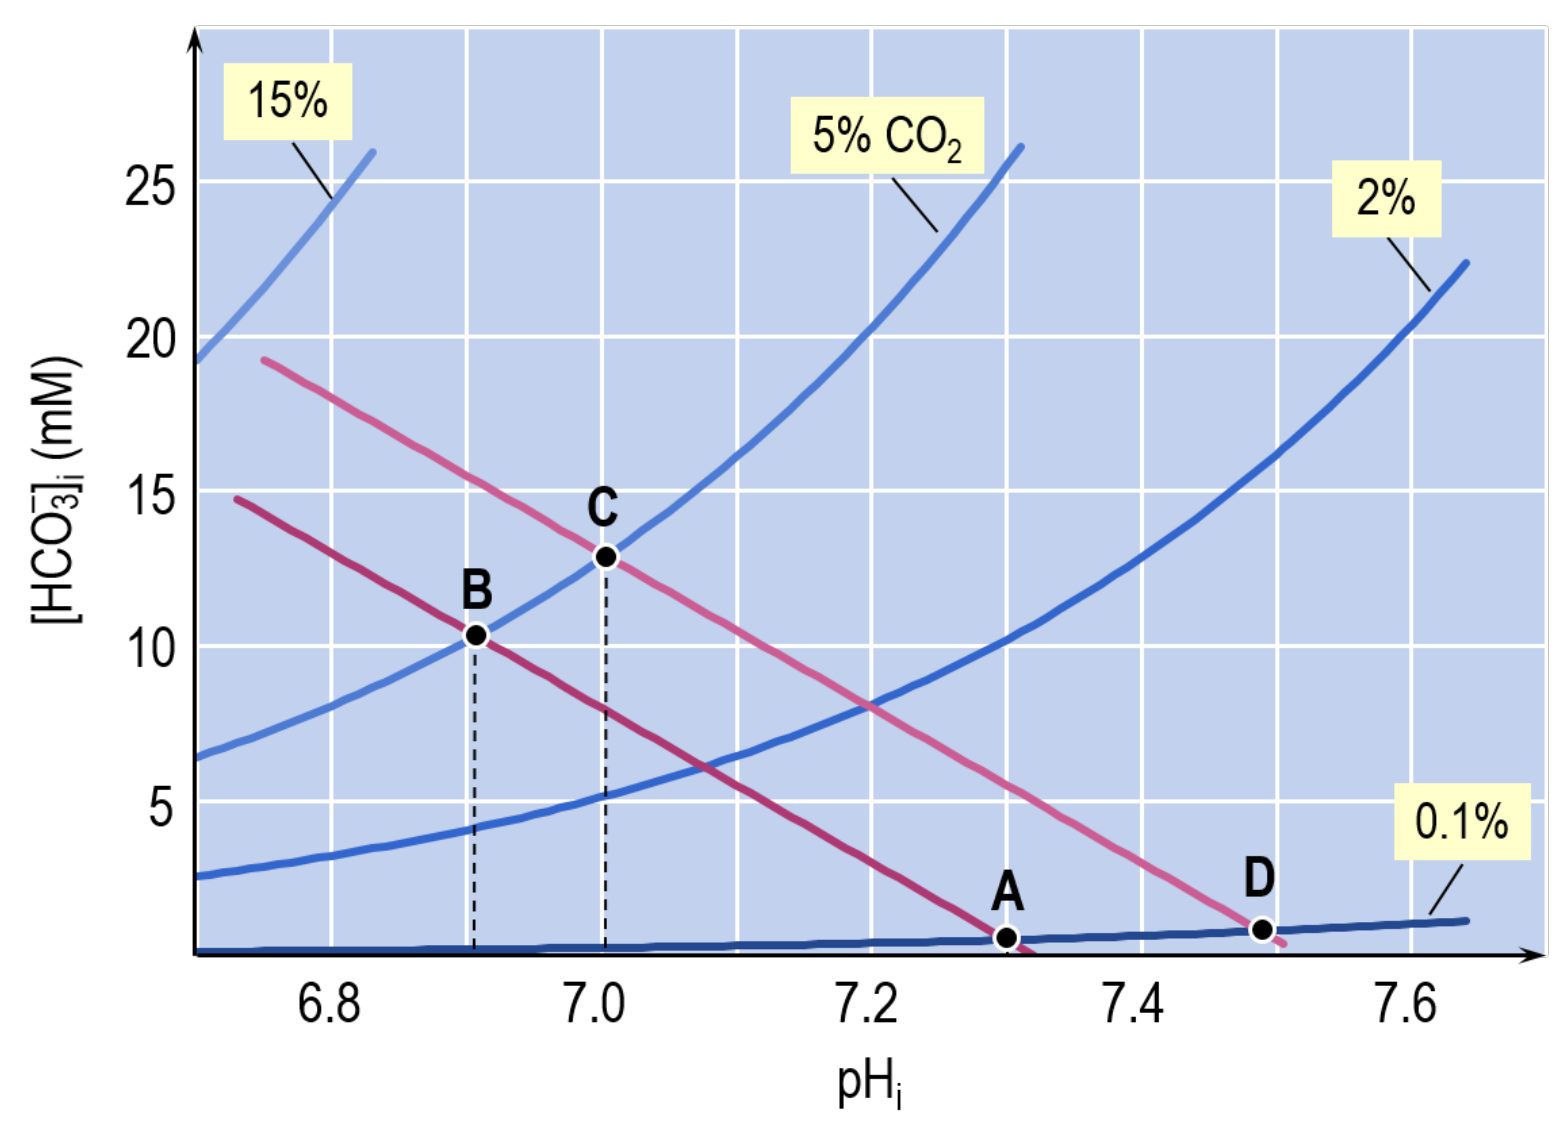
\includegraphics[width=0.5\linewidth]{img/Figure 7.png}
\caption{\label{fig:7} A Davenport diagram (from figure 5A of BDW). This nomogram consists of two kinds of plots. The first kind of plot is represented by the four $\mathrm{CO_2}$ isopleths that slope upwards from left to right. Each isolpleth represents all possible combinations of $\mathrm{[HCO_3^-]_i}$ and $\mathrm{pH_i}$ for a given $\mathrm{[CO_2]_i}$ (described here as the $\%$ of the air phase that is $\mathrm{CO_2}$). The second kind of plot is represented by the two lines that slope downwards from left to right. The slope of these parallel lines describes the buffering power of non-$\mathrm{CO_2}/\mathrm{HCO_3^-}$ buffers. BDW assumed that the experiment starts at point A, at $\mathrm{pH_i} = 7.32$ and $0.1\%$ $\mathrm{CO_2}$. The addition of $5\%$ $\mathrm{CO_2}$ causes the $\mathrm{pH_i}$ at equilibrium to fall to the point represented by point B. The extrusion of acid during the $\mathrm{CO_2}/\mathrm{HCO_3^-}$ exposure causes the system to move along the $5\%$ $\mathrm{CO_2}$ isopleth from point B to point C. Finally, upon removal of $\mathrm{CO_2}/\mathrm{HCO_3^-}$, the system returns to the original $\mathrm{CO_2}/\mathrm{HCO_3^-}$ isopleth, but now at point D. The difference between points D and A represents the $\mathrm{pH_i}$ overshoot. In the BDW paper, $\beta$ --- the slope of the lines in this figure --- appeared to be $25$ $\mathrm{mM}/\mathrm{pH}$ unit. In fact, the value of $\beta$ determined in the $\mathrm{NH_3}/\mathrm{NH_4^+}$ experiments (also shown as a Davenport-like diagram in figure 5B of BDW) was $9$ $\mathrm{mM}/\mathrm{pH}$ unit. The reason for this discrepancy was probably that BDW delivered the $\mathrm{CO_2}/\mathrm{HCO_3^-}$ solution to the axon using a peristaltic pump and Silastic tubing, which they later realised has a high $\mathrm{CO_2}$ permeability. Thus, the $\mathrm{[CO_2]}$ reaching the axon was $<5\%$, accounting for the artificially inflated value for $\beta$. In their follow-up paper \citep{boron1976intracellular}, BDW delivered the $\mathrm{CO_2}/\mathrm{HCO_3^-}$ solutions from glass syringes and through Saran tubing, which has an extremely low $\mathrm{CO_2}$ permeability.}
\end{figure}

The Davenport diagram traces its origins to the analyses of blood by several eminent investigators about a century ago. It was \cite{henderson1921blood} --- as far as we are able to ascertain --- who in figure 4 of his paper was the first to plot $\mathrm{[HCO_3^-]}$ vs $\mathrm{pH}$ for two $\mathrm{H_2CO_3}$ (rather than $\mathrm{CO_2}$) isopleths, and for two different values of $\beta_\mathrm{non-HCO_3^-}$ (\emph{i.e.}, those produced by $10\%$ and $100\%$ $\mathrm{HbO_2}$).

The power of the Davenport approach is that, knowing the initial conditions and the $\mathrm{pH}$ dependence of $\beta_\mathrm{non-HCO_3^-}$, one can compute with fair accuracy (using the nomogram) or great accuracy (using a computer to solve the equations numerically) the result of virtually any acid-base disorder in the pathophysiological range for a system containing $\mathrm{CO_2}/\mathrm{HCO_3^-}$ and a mixture of non-$\mathrm{HCO_3^-}$ buffers. In their figure 5A (reproduced here as \autoref{fig:7}), BDW used a Davenport approach to describe the initial steady state of a squid giant axon (point A at $\mathrm{pH_i} \approx7.32$, $\mathrm{[CO_2]_i} = 0.1\%$), the initial effect of an exposure to increased $\mathrm{[CO_2]_i}$ (point B, an example of intracellular respiratory acidosis), the effect of the plateau-phase $\mathrm{pH_i}$ recovery (point C, an example of intracellular compensatory metabolic alkalosis), and finally the effect of removing extracellular $\mathrm{CO_2}$ (point D, an example of metabolic alkalosis) to account for the $\mathrm{pH_i}$  overshoot. If one does not know $\beta_\mathrm{non-HCO_3^-}$, the Davenport diagram allows one to compute it from the initial and final $\mathrm{pH}$ . The numerical integration of the BDW equations --- when $P_\mathrm{HCO_3^-}$ and the acid extrusion rate are both zero --- should in principle yield, at infinite time, results consistent with the Davenport diagram.

In their paper (their figure 5B), BDW introduced a novel Davenport-like diagram for the $\mathrm{NH_3}/\mathrm{NH_4^+}$ buffer system, with $\mathrm{[NH_4^+]}$ on the ordinate (replacing $\mathrm{[HCO_3^-]}$), $\mathrm{NH_3}$ isopleths (replacing $\mathrm{CO_2}$ isopleths), and a line describing non-$\mathrm{NH_3}/\mathrm{NH_4^+}$ buffering power (replacing the line describing non-$\mathrm{CO_2}/\mathrm{HCO_3^-}$ buffering power). Like the classical Davenport diagram, this one (or others like it, constructed for other buffer pairs) can be a useful tool for interpreting --- in the steady state --- problems in acid-base chemistry.

In the Davenport analysis, the initial and final conditions represent equilibria. Davenport-like diagrams provides no information about the time course of $\mathrm{pH}$ between the initial and final states. Nor can Davenport-like diagrams deal with time course, barriers (\emph{e.g.}, cell membranes), permeabilities to substances other than the neutral molecule (\emph{e.g.}, $\mathrm{CO_2}$, $\mathrm{NH_3}$), or active transport. Of course, in their pioneering work, Henderson, Davenport, and other authors contributing to this nomogram had no reason to contemplate these future complexities.

\subsection{Pre-BDW Analyses of Transmembrane Distributions of Weak Acids and Bases}

As summarised by \cite{roos1981intracellular}, about a century ago, several authors --- who assumed that $\mathrm{CO_2}$ equilibrates across the plasma membrane but that $\mathrm{HCO_3^-}$ is impermeant --- used the sum $\mathrm{[CO_2]_i}+\mathrm{[HCO_3^-]_i}$ to compute the steady-state $\mathrm{pH_i}$ of several cell types. Then, beginning in 1940, a series of authors introduced three successively more sophisticated mathematical analyses for the steady-state transmembrane distribution of a neutral weak acid and its anionic conjugate weak base (\emph{i.e.}, $\mathrm{TA}$), and three more for the distribution of a neutral weak base and its cationic, conjugate weak acid (\emph{i.e.}, $\mathrm{TB}$). We will now present these analyses in order of increasing complexity, and according to their sequence in time (see \autoref{fig:8}). They all have in common the assumption that the system is either in equilibrium or at least in a steady state supported by the input of energy.

\begin{figure}[ht]
\centering
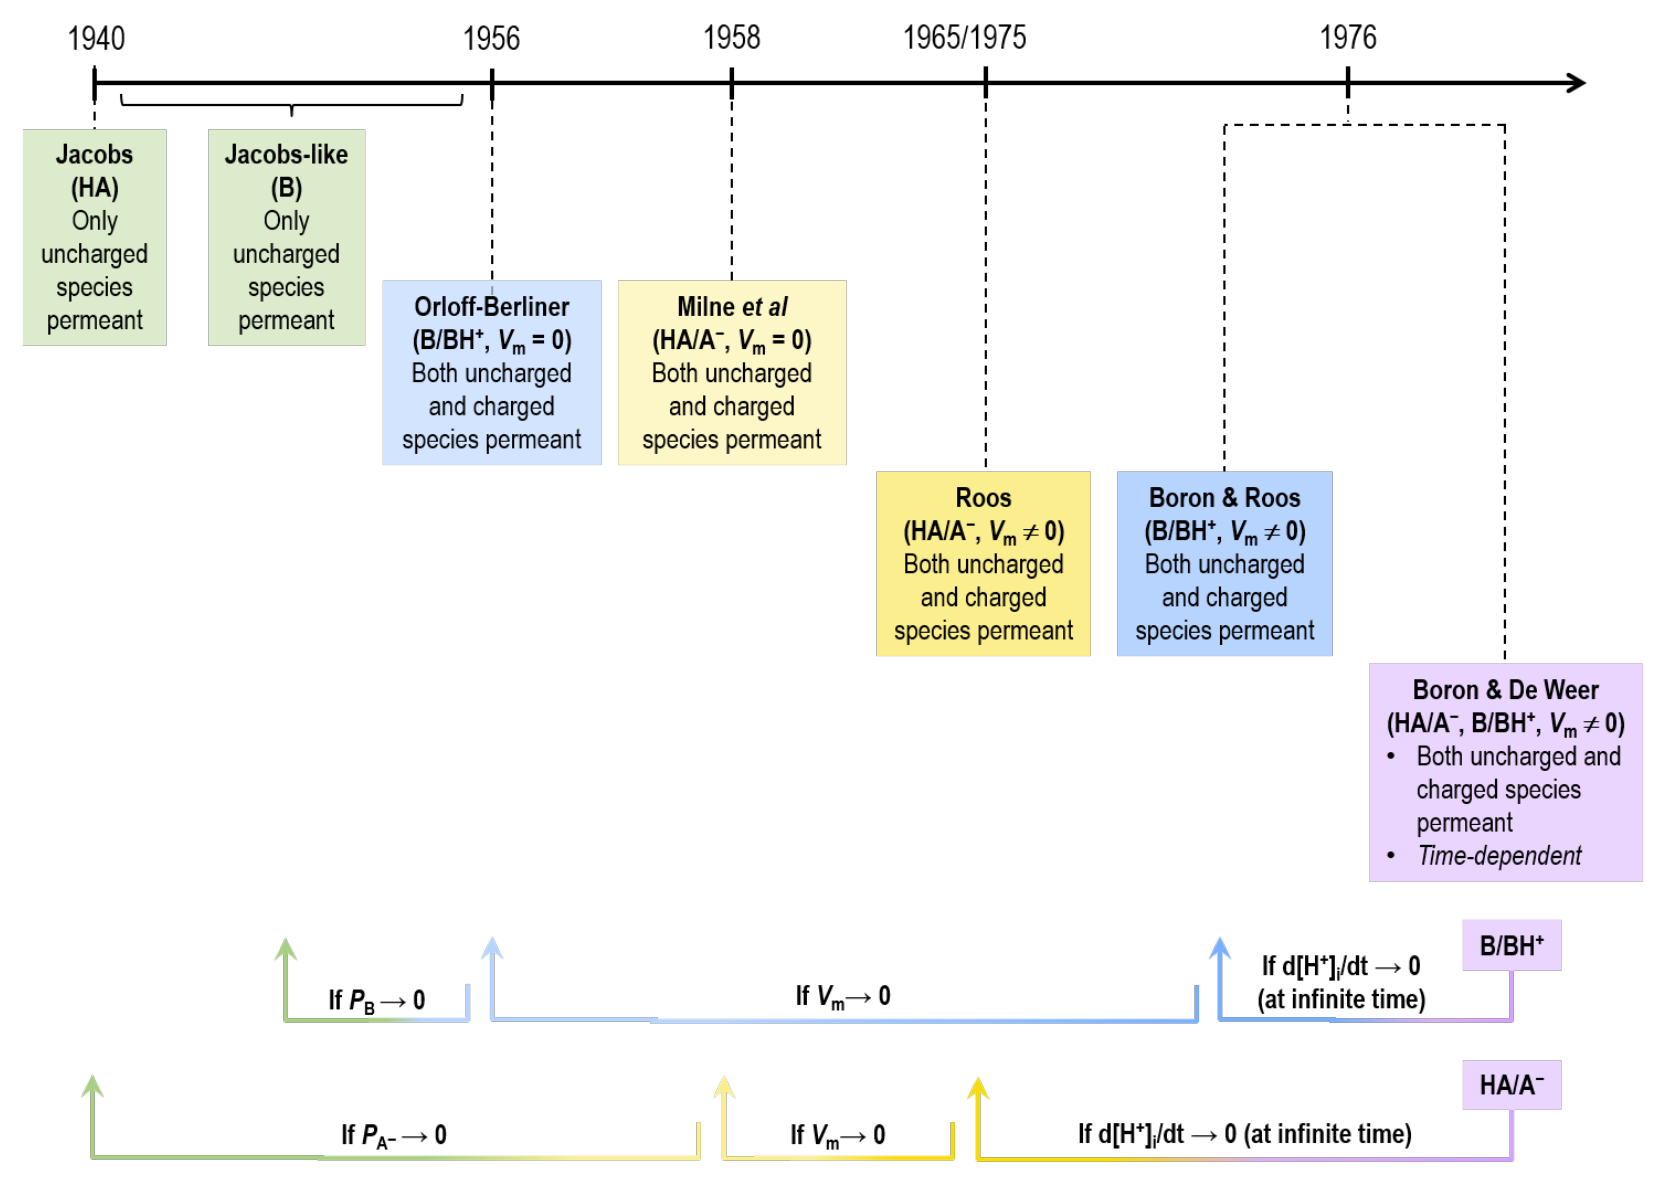
\includegraphics[width=0.8\linewidth]{img/Figure 8.png}
\caption{\label{fig:8} Timeline of acid-base/$\mathrm{pH}$ models prior to BDW. Note that the time-dependent BDW model of weak acid/conjugate weak base ($\mathrm{HA}/\mathrm{A^-}$) collapses to \cite{roos1965intracellular,roos1975intracellular} steady-state model for $\mathrm{HA}/\mathrm{A^-}$. The \cite{roos1965intracellular,roos1975intracellular} model, in turn, reduces to the \cite{milne1958non} model for $\mathrm{HA}/\mathrm{A^-}$ when the membrane potential ($V_\mathrm{m}$) approaches zero. Finally, the \cite{milne1958non} model reduces to the \cite{jacobs1940some} model --- where only one uncharged species $\mathrm{HA}$ is permeant --- as the permeability of $\mathrm{A^-}$ ($P_\mathrm{A^-}$) approaches zero. Similarly, the time-dependent BDW model of weak base/conjugate weak acid ($\mathrm{B}/\mathrm{BH^+}$) collapses to \cite{boron1976comparison} steady-state model for $\mathrm{B}/\mathrm{BH^+}$. The \cite{boron1976comparison} model in turn reduces to the \cite{orloff1956mechanism} model for $\mathrm{B}/\mathrm{BH^+}$ when $V_\mathrm{m}$ approaches zero. Finally, the \cite{orloff1956mechanism} model reduces to the Jacobs-like model --- where only one uncharged species $\mathrm{B}$ is permeant --- as ($P_\mathrm{B}$) approaches zero.}
\end{figure}

\paragraph{Jacobs ($\mathrm{HA}$, neutral weak acid).}

\cite{jacobs1940some} presented a general mathematical model that describes the equilibrium transmembrane distribution of total weak acid ($\mathrm{TA}$), assuming that only the neutral species ($\mathrm{HA}$), but not the conjugate weak base ($\mathrm{A^-}$) can cross the membrane:
\begin{equation}
\dfrac{\mathrm{[TA]_i}}{\mathrm{[TA]_o}}=\dfrac{10^{\mathrm{pH_i}-\mathrm{pK}}+1}{10^{\mathrm{pH_o}-\mathrm{pK}}+1}.
\label{eqn:jacobs}
\end{equation}
In an accompanying document, we show the derivation of the above equation\footnote{See equation 24 in Derivation of the Jacobs Neutral Weak Acid Equation (Log) in Supplementary Files}, the linear form of which is:
\begin{equation}
\dfrac{\mathrm{[TA]_i}}{\mathrm{[TA]_o}}=\left(\dfrac{\mathrm{[H^+]_i}+\mathrm{K}}{\mathrm{[H^+]_o}+\mathrm{K}}\right)\left( \dfrac{\mathrm{[H^+]_o}}{\mathrm{[H^+]_i}}\right).
\label{eqn:jacobs2}
\end{equation}
We also present the derivation of this linear version in an accompanying document\footnote{See equation 25 in Derivation of the Jacobs Neutral Weak Acid Equation (Linear) in Supplementary Files}. A major assumption in the derivations of both \autoref{eqn:jacobs} and \autoref{eqn:jacobs2} is that $\mathrm{HA}$ does not merely move but fully equilibrates across the cell membrane. That is, the system is in equilibrium.

The notion that only the neutral member of the buffer species (\emph{i.e.}, $\mathrm{HA}$) can traverse the membrane is known as nonionic diffusion. \autoref{eqn:jacobs} and \autoref{eqn:jacobs2} tell us that, as $\mathrm{pH_i}$ rises (\emph{i.e.}, $\mathrm{[H^+]_i}$ falls), $\mathrm{[TA]_i}$ rises steeply because $\mathrm{[A^-]_i}$ rises exponentially with $\mathrm{pH_i}$ --- a concept known as ``trapping'' (of the $\mathrm{A^-}$).

\paragraph{Jacobs-like equation ($\mathrm{B}$, neutral weak base).}

Although Jacobs did not present the analogous equation for total weak base ($\mathrm{TB}$), others have derived it, including \cite{roos1981intracellular}:
\begin{equation}
\dfrac{\mathrm{[TB]_i}}{\mathrm{[TB]_o}}=\dfrac{10^{\mathrm{pK}-\mathrm{pH_i}}+1}{10^{\mathrm{pK}-\mathrm{pH_o}}+1}.
\label{eqn:jacobs3}
\end{equation}
In an accompanying document, we show the derivation of \autoref{eqn:jacobs3},\footnote{See equation 33 in Derivation of a Jacobs-like Equation (Log) for a Neutral Weak Base in Supplementary Files} the linear form of which is:
\begin{equation}
\dfrac{\mathrm{[TB]_i}}{\mathrm{[TB]_o}}=\dfrac{\mathrm{[H^+]_i}+\mathrm{K}}{\mathrm{[H^+]_o}+\mathrm{K}}.
\label{eqn:jacobs4}
\end{equation}
We also present a derivation of \autoref{eqn:jacobs4}.\footnote{See equation 21 in Derivation of a Jacobs-like Equation (Linear) for a Neutral Weak Base in Supplementary Files} A major assumption in the derivations of \autoref{eqn:jacobs3} and \autoref{eqn:jacobs4} --- analogous to the situation for \autoref{eqn:jacobs} and \autoref{eqn:jacobs2} --- is that $\mathrm{B}$ fully equilibrates across the cell membrane. That is, the system is in equilibrium.

The notion that only the neutral member of the buffer species (\emph{i.e.}, $\mathrm{B}$) can traverse the membrane is another example of nonionic diffusion. \autoref{eqn:jacobs3} and \autoref{eqn:jacobs4} tell us that, as $\mathrm{pH_i}$ falls (\emph{i.e.}, $\mathrm{[H^+]_i}$ rises), $\mathrm{[TB]_i}$ rises steeply because $\mathrm{[BH^+]_i}$ rises exponentially with the decrease in $\mathrm{pH_i}$ --- another example of ``trapping'' (of the $\mathrm{BH^+}$). Such trapping is especially important in renal physiology, where acidic fluid in renal tubules can trap the cationic form of a buffer pair (\emph{e.g.}, $\mathrm{NH_4^+}$).

\autoref{eqn:jacobs} and \autoref{eqn:jacobs3} provide the theoretical foundation for using $\mathrm{[TA]_i}/\mathrm{[TA]_o}$ ratios for permeant weak acids (\emph{e.g.}, $\mathrm{CO_2}$, above, and the later 5,5'-dimethyl-2,4-oxazolidinedione [DMO] technique) or $\mathrm{[TB]_i}/\mathrm{[TB]_o}$ ratios for permeant weak bases (\emph{e.g.}, for methylamine; see \cite{boron1976comparison}) for computing steady-state $\mathrm{pH_i}$. For example, equation  tells us that, as $\mathrm{pH_i}$ rises, $\mathrm{[TA]_i}/\mathrm{[TA]_o}$ will rise nearly exponentially; this occurs because $\mathrm{[A^-]_i}$ rises in a precisely exponential fashion.

\paragraph{Orloff \& Berliner ($\mathrm{B}/\mathrm{BH^+}$, $V_\mathrm{m}=0$).}

\cite{orloff1956mechanism} extended the Jacobs-like model to a neutral weak base and its cationic conjugate weak acid by permitting not just $\mathrm{B}$ but also $\mathrm{BH^+}$ to permeate a barrier separating compartments 1 and 2. They avoided the complication of $\mathrm{BH^+}$ electrodiffusion by assuming a transmembrane voltage of zero (\emph{i.e.}, $V_\mathrm{m}=0$). Because they recognised that the flux of $\mathrm{BH^+}$ across the barrier would cause $\mathrm{pH}$ to drift in opposite directions in the two compartments, they assumed that independent, energy-requiring processes would stabilise $\mathrm{pH}$ in the two compartments and establish a steady state described by
\begin{equation}
\dfrac{P_\mathrm{B}}{P_\mathrm{BH^+}}=\dfrac{\mathrm{[BH^+]_i}-\mathrm{[BH^+]_o}}{\mathrm{[B]_o}-\mathrm{[B]_i}}.
\label{eqn:orloff}
\end{equation}
In an accompanying document\footnote{See equation 26 in Derivation of the Orloff-Berliner Equation in Supplementary Files}, we show the derivation of \autoref{eqn:orloff}. If we put \autoref{eqn:orloff} into the same form as \autoref{eqn:jacobs4}, which expresses the buffer concentrations in terms of $\mathrm{[TB]_i}$ and $\mathrm{[TB]_o}$ then --- for cells --- we have
\begin{equation}
\dfrac{\mathrm{[TB]_i}}{\mathrm{[TB]_o}}=\left(\dfrac{\mathrm{[H^+]_i}+\mathrm{K}}{\mathrm{[H^+]_o}+\mathrm{K}}\right)\left( \dfrac{\dfrac{P_\mathrm{B}}{P_\mathrm{BH^+}}\mathrm{K}+\mathrm{[H^+]_o}}{\dfrac{P_\mathrm{B}}{P_\mathrm{BH^+}}\mathrm{K}+\mathrm{[H^+]_i}}\right).
\label{eqn:orloff2}
\end{equation}
As $P_\mathrm{BH^+}$ approaches zero, \autoref{eqn:orloff2} reduces to \autoref{eqn:jacobs4} --- the Jacobs-like equation for a weak base. The accompanying document\footnote{See equation 55 in Derivation of the Orloff-Berliner Equation in Supplementary Files} also shows the derivation of \autoref{eqn:orloff2}, as well as the mathematics that shows the limit of this expression as $P_\mathrm{BH^+}$ approaches zero.

Note that the flux of $\mathrm{BH^+}$ --- which leads to a flux of $\mathrm{B}$ in the opposite direction --- tends to push the system off equilibrium. As noted above, the Orloff-Berliner equation requires that the system be in a steady-state, which can be achieved, as they recognised, only by an input of energy to maintain all relevant concentrations constant over time.

\paragraph{Milne et al ($\mathrm{HA}/\mathrm{A^-}$, $V_\mathrm{m}=0$).}

Milne and colleagues (1958) developed a steady-state expression similar to that of Orloff \& Berliner, but for the transmembrane distribution of a neutral weak acid and its anionic conjugate weak:
\begin{equation}
\dfrac{P_\mathrm{HA}}{P_\mathrm{A^-}}=\dfrac{\mathrm{[A^-]_i}-\mathrm{[A^-]_o}}{\mathrm{[HA]_o}-\mathrm{[HA]_i}}.
\label{eqn:milne}
\end{equation}
An accompanying document\footnote{See equation 26 in Derivation of the Equation of Milne et al for a Neutral Weak Acid in Supplementary Files} shows the derivation of \autoref{eqn:milne}, which we can also put in the form of \autoref{eqn:orloff2}, which expresses buffer concentrations in terms of $\mathrm{[TA]_i}$ and $\mathrm{[TA]_o}$:
\begin{equation}
\dfrac{\mathrm{[TA]_i}}{\mathrm{[TA]_o}}=\left(\dfrac{\mathrm{[H^+]_i}+\mathrm{K}}{\mathrm{[H^+]_o}+\mathrm{K}}\right)\left( \dfrac{\dfrac{P_\mathrm{HA}}{P_\mathrm{A^-}}\mathrm{[H^+]_o}+\mathrm{K}}{\dfrac{P_\mathrm{HA}}{P_\mathrm{A^-}}\mathrm{[H^+]_i}+\mathrm{K}}\right).
\label{eqn:milne2}
\end{equation}
As $P_\mathrm{A^-}$ approaches zero, \autoref{eqn:milne2} reduces to \autoref{eqn:jacobs2} --- the Jacobs equation for a weak acid. The accompanying document\footnote{See equation 62 in Derivation of the Equation of Milne et al for a Neutral Weak Acid in Supplementary Files} also shows the derivation of \autoref{eqn:milne2}, as well as the mathematics that shows the limit of this expression as $P_\mathrm{A^-}$ approaches zero.

\paragraph{Roos ($\mathrm{HA}/\mathrm{A^-}$, non-zero $V_\mathrm{m}$).}

In 1965 and 1975, Roos extended the Irvine model by allowing $V_\mathrm{m}$ to assume non-zero values \citep{roos1965intracellular,roos1975intracellular}, and derived the following equation,
\begin{equation}
\dfrac{\mathrm{[TA]_i}}{\mathrm{[TA]_o}}=\left(\dfrac{\mathrm{[H^+]_i}+\mathrm{K}}{\mathrm{[H^+]_o}+\mathrm{K}}\right)\left( \dfrac{\dfrac{P_\mathrm{HA}}{P_\mathrm{A^-}}\mathrm{[H^+]_o}+\dfrac{FV_\mathrm{m}}{RT(1-\epsilon)}\mathrm{K}}{\dfrac{P_\mathrm{HA}}{P_\mathrm{A^-}}\mathrm{[H^+]_i}+\dfrac{FV_\mathrm{m}}{RT(1-\epsilon)}\mathrm{K}}\right),
\label{eqn:roos}
\end{equation}
where $\epsilon$ has the same meaning as in the derivation of the BDW equations: $e^{-V_\mathrm{m}F/RT}$. An accompanying document\footnote{See equation 45 in Derivation of the Roos Equation in Supplementary Files} shows the derivation of \autoref{eqn:roos}. This document also shows that, at the limits of certain parameters, \autoref{eqn:roos} simplifies to the expected equation:

\begin{enumerate}[noitemsep] 
\item As $V_\mathrm{m} \rightarrow 0$, the Roos equation simplifies to the equation of Milne et al (which assumes $V_\mathrm{m}=0$).

\item As $P_\mathrm{A^-} \rightarrow 0$, the Roos equation simplifies to the Jacobs equation (which assumes $P_\mathrm{A^-}=0$).

\item As $P_\mathrm{HA} \rightarrow 0$, the Roos equation simplifies to the Nernst equation (which assumes permeability to only $\mathrm{A^-}$).
\end{enumerate}

The Roos equation was important historically because it allowed one to assess possible errors in $\mathrm{pH_i}$ values computed from the transmembrane distribution of a neutral weak acid (\emph{e.g.}, $\mathrm{CO_2}$, DMO) and its monovalent anion conjugate weak base. These errors could in principle arise from membrane permeability to $\mathrm{A^-}$ (as already considered by Milne et al), as influenced by $V_\mathrm{m}$.

\paragraph{Boron \& Roos ($\mathrm{B}/\mathrm{BH^+}$, non-zero $V_\mathrm{m}$).}

Finally, \cite{boron1976comparison} derived an equation similar to the Roos equation, but for the distribution of a neutral weak base and its monovalent cationic conjugate weak acid:
\begin{equation}
\dfrac{\mathrm{[TB]_i}}{\mathrm{[TB]_o}}=\left(\dfrac{\mathrm{[H^+]_i}+\mathrm{K}}{\mathrm{[H^+]_o}+\mathrm{K}}\right)\left( \dfrac{\dfrac{P_\mathrm{B}}{P_\mathrm{BH^+}}\mathrm{K}+\dfrac{FV_\mathrm{m}}{RT(\epsilon '-1)}\mathrm{[H^+]_o}}{\dfrac{P_\mathrm{B}}{P_\mathrm{BH^+}}\mathrm{K}+\dfrac{FV_\mathrm{m}}{RT(\epsilon '-1)}\epsilon '\mathrm{[H^+]_i}}\right),
\label{eqn:roos2}
\end{equation}
where $\epsilon '$ has the same meaning as in the derivation of the BDW equations: $e^{V_\mathrm{m}F/RT}$. An accompanying document\footnote{See equation 44 in Derivation of the Boron-Roos Equation in Supplementary Files} shows the derivation of \autoref{eqn:roos2}. This document also shows that, at the limits of certain parameters, \autoref{eqn:roos2} simplifies to the expected equation:

\begin{enumerate}[noitemsep] 
\item As $V_\mathrm{m} \rightarrow 0$, the Boron-Roos equation simplifies to the equation of Orloff \& Berliner (which assumes $V_\mathrm{m}=0$).
\item As $P_\mathrm{BH^+} \rightarrow 0$, the Boron-Roos equation simplifies to the Jacobs-like equation for a neutral weak base (which assumes $P_\mathrm{BH^+}=0$).
\item As $P_\mathrm{B}=0$, the Boron-Roos equation simplifies to the Nernst equation (which assumes permeability to only $\mathrm{BH^+}$).
\end{enumerate}

The Boron-Roos equation was important historically because it allowed one to assess possible errors in $\mathrm{pH_i}$ values computed from the transmembrane distribution of a neutral weak base (\emph{e.g.}, methylamine) and its monovalent anion conjugate weak base. These errors could in principle arise from membrane permeability to $\mathrm{BH^+}$, as influenced by $V_\mathrm{m}$. In their paper, Boron and Roos used the transmembrane distribution of methylamine/methylammonium to monitor a downward drift in $\mathrm{pH_i}$ caused by the passive influx of methylammonium. This was the first use of a chemical-distribution technique to follow $\mathrm{pH_i}$ changes over time.

We have already noted for the Orloff-Berliner equation that the derivation requires that the system be in a steady-state, which can be achieved only by an input of energy to maintain all relevant concentrations constant over time. The same is true for the equations of Milne et al, Roos, and Boron \& Roos.

\subsection{Comparison of the Pre-BDW Analyses with the BDW Equations}

The BDW equations build on the earlier work on buffering and transmembrane distributions of weak acids and bases, presented in the previous two sections. Of course, the work of Koppel and Spiro, and Van Slyke, as well as their predecessors who developed the physico-chemical principles of acid-base chemistry, is at the heart of the BDW model.

An important aspect of the Davenport diagram is its predictive power. For example, given $\beta_\mathrm{non-HCO_3^-}$ as well as the initial $\mathrm{pH}$ and $\mathrm{[CO_2]}$, the Davenport approach can predict the effect of an increase in $\mathrm{[CO_2]}$ on the final equilibrium conditions. However, the Davenport approach makes no statement about mechanism or time course. The BDW approach has all the predictive power of Davenport, but also addresses mechanism and time course.

The six pre-BDW approaches for assessing transmembrane distributions of $\mathrm{HA}/\mathrm{A^-}$ and $\mathrm{B}/\mathrm{BH^+}$ all start with the weak acid/base present and the system in an equilibrium or at least in a steady state. Somehow, the system --- the cell and its surrounding fluid --- went from a condition with no weak acid/base present to a condition with the weak acid/base present at equilibrium/steady state. The older models make no attempt to describe how and how fast the system achieved the new state, and --- unlike the Davenport approach --- have no predictive value for relating initial and final conditions. It is worth noting that the investigators who developed these six approaches were interested mainly in using tracer levels of weak acids/bases to compute $\mathrm{pH_i}$. The intention was that tracer levels would have minimal effects on the state of the system --- hence, the minimal interest in the prediction. Note that, at infinite time (and with no acid extrusion), the BDW equations reduce to those six transmembrane-distribution analyses presented in the previous section.

To some extent, the BDW models represent a merger of the Davenport and the six pre-BDW approaches for assessing transmembrane distributions of $\mathrm{HA}/\mathrm{A^-}$ and $\mathrm{B}/\mathrm{BH^+}$. Like the Davenport approach, the BDW approach is predictive. However, unlike Davenport's approach, the BDW models provide insight into mechanism and time course, and are applicable even when the system is far from equilibrium/steady state. Like the six transmembrane-distribution models, the BDW models provide insight into how $\mathrm{pH_i}$ and $V_\mathrm{m}$ affect $\mathrm{[HA]_i}$, $\mathrm{[A^-]_i}$, $\mathrm{[B]_i}$, and $\mathrm{[BH^+]_i}$. Unlike the six transmembrane-distribution models, the BDW models are predictive and provide insight into mechanism and time course.

It is worth noting that BDW derived their equations under the influence of Albert Roos, who had derived the transmembrane-distribution model for $\mathrm{HA}/\mathrm{A^-}$ \citep{roos1975intracellular} and who inspired Boron's derivation of the $\mathrm{B}/\mathrm{BH^+}$ model \citep{boron1976comparison}.

\subsection{Post-BDW Development of Concepts}
\paragraph{Fundamental law of $\mathrm{pH_i}$ regulation.}

Recall that one of the intermediate steps of the derivation of the BDW equations for the $\mathrm{HA}/\mathrm{A^-}$ system was \autoref{eqn:pH_rate2}, which we reproduce here:
\begin{equation}
\dfrac{\mathrm{dpH}}{\mathrm{dt}} = \left(\dfrac{-1}{\beta}\right)\left(\dfrac{\mathrm{dQ}}{\mathrm{dt}}\right). 
\end{equation}
Another intermediate step was the description of $\mathrm{d}Q/\mathrm{d}t$ in \autoref{eqn:Q_rate2}, which we reproduce here:
\begin{equation}
\dfrac{\mathrm{d}Q}{\mathrm{d}t}=\rho\Big( (1-\alpha)J_\mathrm{HA}-\alpha J_{\mathrm{A^-}}-J_\mathrm{H^+} \Big).
\end{equation}
Combining the above two equations yields a primitive form of the fundamental law of $\mathrm{pH_i}$ regulation:
\begin{equation}
\dfrac{\mathrm{dpH_i}}{\mathrm{d}t}=-\dfrac{1}{\beta}\underbrace{\rho \Big( {(1-\alpha)J_\mathrm{HA}}-{\alpha J_\mathrm{A^-}-J_\mathrm{H^+}} \Big) }_{{\mathrm{d}Q}/{\mathrm{d}t}}.
\label{eqn:fund}
\end{equation}
In the later literature, Boron and colleagues in effect dissected the $\mathrm{d}Q/\mathrm{d}t$ term --- the net rate at which $\mathrm{H^+}$ appear in the cytosol ($\mathrm{mol\cdot m^{-3}\cdot s^{-1}}$) --- into two concepts that are more general than those considered by BDW in \autoref{eqn:fund}: the intracellular acid-loading rate ($J_L$) and the intracellular acid-extrusion rate ($J_E$).

In the narrow definition of \autoref{eqn:fund} the only $J_L$ term is $(1-\alpha)J_\mathrm{HA}$. In the post-BDW literature, Boron and colleagues defined $J_L$ to comprise every process that adds the equivalent of $\mathrm{H^+}$ to or removes the equivalent of $\mathrm{OH^-}$ from the cytosol, including $\mathrm{H^+}$ channels (mediating passive $\mathrm{H^+}$ influx), a variety of transporters (\emph{e.g.}, $\mathrm{Cl}$-$\mathrm{HCO_3}$ exchangers mediating $\mathrm{HCO_3^-}$ efflux), and the metabolic production of acid. \cite{boron1979ph} measured and introduced the term ``rate of acid introduction''. \cite{roos1981intracellular} later replaced this term when they coined ``acid-loading rate''.

In the narrow definition of \autoref{eqn:fund}, the $J_E$ terms are $\alpha J_\mathrm{A^-}$ and $J_\mathrm{H^+}$. Note that BDW defined $J_\mathrm{H^+}$ as the $\mathrm{H^+}$-extrusion rate above baseline. In the post-BDW literature, Boron and colleagues defined $J_E$ to comprise every process that removes the equivalent of $\mathrm{H^+}$ from or adds the equivalent of $\mathrm{OH^-}$ to the cytosol, including a variety of transporters (\emph{e.g.}, $\mathrm{H^+}$ pumps, $\mathrm{Na}$-$\mathrm{H}$ exchangers) that mediate $\mathrm{H^+}$ efflux and others (\emph{e.g.}, $\mathrm{Na^+}$-driven $\mathrm{HCO_3^-}$ transporters, $\mathrm{H^+}/\mathrm{lactate}$ cotransporters) that mediate base efflux. It appears that Boron in 1977 provided the first definition of acid extrusion.

Recasting \autoref{eqn:fund} in terms of $J_L$ and $J_E$,
\begin{equation}
\dfrac{\mathrm{dpH_i}}{\mathrm{d}t}=-\dfrac{1}{\beta}\underbrace{\rho\Big(\underbrace{(1-\alpha)J_\mathrm{HA}}_{J_\mathrm{L}~\mathrm{term}}\underbrace{-\alpha J_\mathrm{A^-}-J_\mathrm{H^+}}_{J_\mathrm{E}~\mathrm{terms}}\Big)}_{{\mathrm{d}Q}/{\mathrm{d}t}}.
\label{eqn:fund1}
\end{equation}
The modern version of the fundamental law of $\mathrm{pH_i}$ regulation is:
\begin{equation}
\dfrac{\mathrm{dpH_i}}{\mathrm{d}t}=\dfrac{\rho}{\beta}(J_E-J_L).
\label{eqn:fund2}
\end{equation}
Here, with the explicit inclusion of $\rho$, $J_E$ and $J_L$ have the units ($\mathrm{moles}\cdot\mathrm{cm^{-2}\cdot s^{-1}}$).

\autoref{eqn:fund2} tells us that $\mathrm{pH_i}$ is stable when $J_E=J_L$, rises when $J_E>J_L$, and falls with $J_E<J_L$. BDW did not derive the above equation in their 1976 paper. The first statement of the concept of \autoref{eqn:fund2} was in sentence form in the review by \cite{roos1981intracellular}, who also provided a graphical example in their figure 12. By 1989, Boron presented a version of \autoref{eqn:fund2} that lacks the term $\rho$. Thus, he implicitly defined $J_E$ and $J_L$ in terms of ($\mathrm{moles}\cdot\mathrm{cm^{-3}\cdot s^{-1}}$). This 1989 paper also included examples of how \autoref{eqn:fund2} could help one interpret the time course of $\mathrm{pH_i}$ in many experimental settings. For example, a bolus introduction of acid into a cell --- an ``acute'' intracellular acid load, coined by Boron by the time of this 1989 review --- rapidly lowers $\mathrm{pH_i}$, but also increases $J_E$ and decreases $J_L$. Because $J_E$ now exceeds $J_L$, $\mathrm{pH_i}$ recovers to its initial value. By 1992, Boron coined the term ``fundamental law of $\mathrm{pH_i}$ regulation'' to describe \autoref{eqn:fund2}.

Note that an acute or bolus intracellular acid load is to be distinguished from a chronic intracellular load (the rate of which is $J_L$). The amount of an acute acid load can instantly be quantitated in acid equivalents. The amount of a chronic acid load can only be quantitated in acid equivalents by integrating $J_L$ over time.

Later, \cite{boron2004regulation} provided a more detailed description of $\mathrm{pH_i}$ regulation, as well as a tongue-in-cheek analogy --- which he had been using for years in lectures --- between $\mathrm{pH_i}$ regulation and the temperature regulation of a house, complete with multiple furnaces (acid-extruders), multiple air conditioners (acid loaders), heat capacity (buffering power), a thermostat ($\mathrm{pH_i}$ sensitivity of the transporters), and weather radar (extracellular sensors for $\mathrm{CO_2}$, $\mathrm{HCO_3^-}$, and $\mathrm{pH}$).

\paragraph{Flux vs pseudoflux.}

One can define the acid-loading and acid-extrusion rates as strict fluxes, with units of $\mathrm{moles/(membrane~area~\times~time})$. Such of use of $J_E$ or $J_L$ --- for example $J_\mathrm{NBC}$ (the acid-extruding flux mediated by a $\mathrm{Na}/\mathrm{HCO_3}$ cotransporter, $\mathrm{NBC}$) or $J_\mathrm{Cl-HCO_3}$ (the acid-loading flux mediated by a $\mathrm{Cl}$-$\mathrm{HCO_3}$ exchanger) --- is most appropriate in cases in which the cell has a simple geometry (\emph{e.g.}, a squid axon or \emph{Xenopus} oocyte). However, for cells with complex geometries --- where surface-to-volume ratios are difficult to define --- physiologists often present experimental data in the units ``$\mathrm{moles/(volume~of~cell~water})$''. To avoid confusion between the two systems of measurement, \cite{bevensee1995} introduce the term ``pseudoflux'' and the symbol $\phi$ (rather than $J$). Thus, in their paper, the authors referred to $\phi_E$ and $\phi_L$ (rather than $J_E$ and $J_L$), so that the fundamental law of $\mathrm{pH_i}$ regulation becomes
\begin{equation}
\dfrac{\mathrm{dpH_i}}{\mathrm{d}t}=\dfrac{\phi_E-\phi_L}{\beta}.
\label{eqn:fund3}
\end{equation}

\paragraph{Effect of isodirectional fluxes of $\mathrm{HA}/\mathrm{A^-}$ or $\mathrm{B}/\mathrm{BH^+}$ fluxes on $\mathrm{pH}$ near a membrane.}

The $\alpha$ term in \autoref{eqn:y} and \autoref{eqn:alpha_B}, and the $(1-\alpha)$ term in \autoref{eqn:y2} and \autoref{eqn:alpha_B2} inspired an insight that yields equations analogous to the familiar Henderson-Hasselbalch equation. The starting point was the following question: if both $\mathrm{B}$ and $\mathrm{BH^+}$ cross the membrane in the same direction, how will their isodirectional fluxes affect $\mathrm{pH}$ on the \emph{cis} side (the side from which they depart) and the \emph{trans} side (the side to which they go)?

In the discussion of their paper, \cite{musa2009concentration} showed that if the flux ratio $J_\mathrm{NH_3}/J_\mathrm{NH_4^+}$ is the same as the concentration ratio $\mathrm{[NH_3]_i}/\mathrm{[NH_4^+]_i}$, the flux will have no effect on $\mathrm{pH_i}$ because $\mathrm{NH_3}$ and $\mathrm{NH_4^+}$ are appearing (or disappearing) at the inner surface of the membrane in a proportion equal to their respective, pre-existing concentrations. Similarly, if the flux ratio $J_\mathrm{NH_3}/J_\mathrm{NH_4^+}$ is the same as the concentration ratio $\mathrm{[NH_3]_o}/\mathrm{[NH_4^+]_o}$, the flux will have no effect on $\mathrm{pH_o}$. Stated somewhat differently, as in equation 4 of \cite{musa2009concentration},
\begin{equation}
\mathrm{pH_{i,Null}}=\mathrm{pK_a}+\log \dfrac{J_\mathrm{NH_3}}{J_\mathrm{NH_4^+}},\quad \mathrm{or~ more~ generally},\quad \mathrm{pH_{i,Null}}=\mathrm{pK_a}+\log \dfrac{J_\mathrm{B}}{J_\mathrm{BH^+}}
\label{eqn:phnull}
\end{equation}
and
\begin{equation}
\mathrm{pH_{o,Null}}=\mathrm{pK_a}+\log \dfrac{J_\mathrm{NH_3}}{J_\mathrm{NH_4^+}},\quad \mathrm{or~ more~ generally},\quad \mathrm{pH_{o,Null}}=\mathrm{pK_a}+\log \dfrac{J_\mathrm{B}}{J_\mathrm{BH^+}}
\label{eqn:phnull2}
\end{equation}
Here, $\mathrm{pH_{i,Null}}$ is the $\mathrm{pH_i}$ at which the isodirectional fluxes $J_B$ and $J_\mathrm{BH^+}$ will have no effect on $\mathrm{pH_i}$. Similarly, $\mathrm{pH_{o,Null}}$ is the $\mathrm{pH_o}$ at which the isodirectional fluxes $J_B$ and $J_\mathrm{BH^+}$ will have no effect on $\mathrm{pH_o}$. If $\mathrm{pH_i}$ = $\mathrm{pH_o}$, then their null $\mathrm{pH}$ values are the same (\emph{i.e.}, at this $\mathrm{pH}$, the isodirectional fluxes of $\mathrm{B}$ and $\mathrm{BH^+}$ will have no effect on either $\mathrm{pH}$). One can write equations similar to \autoref{eqn:phnull} and \autoref{eqn:phnull2}, but for $\mathrm{CO_2}$ and $\mathrm{HCO_3^-}$ (or $\mathrm{HA}$ and $\mathrm{A^-}$), which we do here for the first time:
\begin{equation}
\mathrm{pH_{i,Null}}=\mathrm{pK_a}+\log \dfrac{J_\mathrm{HCO_3^-}}{J_\mathrm{CO_2}},\quad \mathrm{or~ more~ generally},\quad \mathrm{pH_{i,Null}}=\mathrm{pK_a}+\log \dfrac{J_\mathrm{A^-}}{J_\mathrm{HA}}
\label{eqn:phnull3}
\end{equation}
and
\begin{equation}
\mathrm{pH_{o,Null}}=\mathrm{pK_a}+\log \dfrac{J_\mathrm{HCO_3^-}}{J_\mathrm{CO_2}},\quad \mathrm{or~ more~ generally},\quad \mathrm{pH_{o,Null}}=\mathrm{pK_a}+\log \dfrac{J_\mathrm{A^-}}{J_\mathrm{HA}}
\label{eqn:phnull4}
\end{equation}
The previous four equations can be valuable for interpreting, for example, the effects of isodirectional fluxes of $\mathrm{CO_2}$ and $\mathrm{HCO_3^-}$. The equations cannot predict the speed or extent of the $\mathrm{pH}$ change, only the direction. For instance, if we expose a cell to a $\mathrm{CO_2}/\mathrm{HCO_3^-}$ solution and $\mathrm{pH_i}$ falls, does mean that $J_\mathrm{CO_2}>J_\mathrm{HCO_3^-}$? The intuitive answer would be, ``yes''. The actual answer is, ``not necessarily''. Imagine that --- in a $\mathrm{CO_2}/\mathrm{HCO_3^-}$-free environment --- we have a $\mathrm{CO_2}/\mathrm{HCO_3^-}$-free cell at a $\mathrm{pH_i}$ of $7.1$. Although no $\mathrm{CO_2}/\mathrm{HCO_3^-}$ is present, we assume that the $\mathrm{pK_a}$ of the $\mathrm{CO_2}/\mathrm{HCO_3^-}$ equilibrium would be $6.1$ if $\mathrm{CO_2}/\mathrm{HCO_3^-}$ were present. We now suddenly add $\mathrm{CO_2}/\mathrm{HCO_3^-}$ to the extracellular fluid --- the precise ratio is of no consequence here because we will focus on the intracellular fluid. $\mathrm{CO_2}$ and $\mathrm{HCO_3^-}$ now begin to enter the cell by any route. If the ratio $J_\mathrm{HCO_3^-}/J_\mathrm{CO_2}= 10^{\mathrm{pH_i}-\mathrm{pK_a}} = 10^{7.1-6.1} = 10$, then $\mathrm{pH_i}$  will not change from its original value of $7.1$ because $\mathrm{HCO_3^-}$ and $\mathrm{CO_2}$ are entering the cell precisely in the correct ratio for a $\mathrm{pH}$ of $7.1$. If $J_\mathrm{HCO_3^-}/J_\mathrm{CO_2}<10$ (in this case), $\mathrm{pH_i}$ will fall because the alkalinising $\mathrm{pH_i}$ effects of the $\mathrm{HCO_3^-}$ influx are less than the acidifying $\mathrm{pH_i}$ effects of the $\mathrm{CO_2}$ influx. This approach cannot tell us how fast or how far $\mathrm{pH_i}$ will fall, only that, initially at least, it must fall. The same analysis can be applied --- simultaneously --- to the extracellular fluid.

\subsection{Post-BDW Models of Acid-Base Fluxes/Chemistry}

Following the development of the BDW model, the field of $\mathrm{pH}$ regulation has seen several modelling efforts. Here, we summarise several, with emphasis on those models that, in our opinion and to the best of our knowledge, have contributed to advance the field, either by extending the BDW model or by introducing new modelling paradigms.

\paragraph{Keifer and Roos.}

In 1981, Keifer and Roos refined the BDW model by modifying the BDW assumption that addition of an infinitesimal amount of weak acid $\mathrm{HA}$ (or $\mathrm{A^-}$, $\mathrm{B}$, or $\mathrm{BH^+}$) during an infinitesimal increment in time does not alter the pre-existing equilibrium ratio $\mathrm{[HA]_i}/\mathrm{[A^-]_i}$ or $\mathrm{[B]_i}/\mathrm{[BH^+]_i}$ \citep{keifer1981membrane}. These authors were interested in the transmembrane fluxes of the neutral weak acid DMO and its conjugate weak base. Keifer \& Roos assumed that --- at the end of the infinitesimal time increment during which $\mathrm{HA}$ and $\mathrm{A^-}$ entered/left the cell --- the cytosolic $\mathrm{HA}$, $\mathrm{A^-}$ and $\mathrm{H^+}$ re-equilibrated. They used this variation on the BDW approach to estimate $P_\mathrm{HA}$ and $P_\mathrm{A^-}$, finding that the plasma membrane permeability to $\mathrm{HA}$ is $\approx 10^3$ higher than to $\mathrm{A^-}$. In the appendix of their paper, Keifer \& Roos derived their refined version of the BDW equations for $\mathrm{HA}/\mathrm{A^-}$:
\begin{equation*}
\dfrac{\mathrm{d[TA]_i}}{\mathrm{d}t}=\rho\left(J_\mathrm{HA}+J_\mathrm{A^-}\right),
\label{eqn:keifer}
\end{equation*}
\begin{equation*}
\dfrac{\mathrm{d[H^+]_i}}{\mathrm{d}t}=\dfrac{2.303\mathrm{[H^+]_i}}{\beta}\rho\left(\left(\dfrac{K_\mathrm{HA}}{\mathrm{[H^+]_i}+K_\mathrm{HA}+{K_\mathrm{new}}}\right)J_\mathrm{HA}-\left(\dfrac{\mathrm{[H^+]_i}}{\mathrm{[H^+]_i}+K_\mathrm{HA}+{K_\mathrm{new}}}\right)J_\mathrm{A^-} \right),
\label{eqn:keifer2}
\end{equation*}
where
\begin{equation*}
K_\mathrm{new}=2.303K_\mathrm{HA}\left( \dfrac{\mathrm{[TA]_i}}{\beta}\right)\left( \dfrac{\mathrm{[H^+]_i}}{\mathrm{[H^+]_i}+K_\mathrm{HA}}\right),
\end{equation*}
\begin{equation*}
J_\mathrm{HA}=P_\mathrm{HA}\left( \mathrm{[HA]_o}-\dfrac{\mathrm{[H^+]_i}}{\mathrm{[H^+]_i}+K_\mathrm{{HA}}}\mathrm{[TA]_i} \right),
\end{equation*}
\begin{equation*}
J_\mathrm{A^-}=P_\mathrm{A^-}\left(\dfrac{V_\mathrm{m}F}{RT}\right)\left(\dfrac{\mathrm{[A^-]_o}-\dfrac{K_\mathrm{HA}}{\mathrm{[H^+]_i}+K_\mathrm{HA}}\mathrm{[TA]_i} \epsilon}{1-\epsilon}\right).
\end{equation*}
The first of these two equations is identical to that presented by BDW, whereas the second includes the new terms ($K_\mathrm{new}$).

In the appendix of their paper, Keifer and Roos noted that it is possible to derive a comparable pair of equations for $\mathrm{B}/\mathrm{BH^+}$. In their 1981 review, Roos \& Boron reported the two equations of the refined BDW model for $\mathrm{B}/\mathrm{BH^+}$ (see their \autoref{eqn:H_rate} and \autoref{eqn:H_rate2}): 
\begin{equation*}
\dfrac{\mathrm{d[TB]_i}}{\mathrm{d}t}=\rho\left(J_\mathrm{B}+J_\mathrm{BH^+} \right),
\label{eqn:keifer2}
\end{equation*}
\begin{equation*}
\dfrac{\mathrm{d[H^+]_i}}{\mathrm{d}t}=\dfrac{2.303\mathrm{[H^+]_i}}{\beta}\rho\left(\left(\dfrac{K_\mathrm{BH^+}}{\mathrm{[H^+]_i}+K_\mathrm{BH^+}+{K_\mathrm{new}}}\right)J_\mathrm{BH^+}-\left(\dfrac{\mathrm{[H^+]_i}}{\mathrm{[H^+]_i}+K_\mathrm{BH^+}+{{K_\mathrm{new}}}}\right)J_\mathrm{B}\right),
\label{eqn:keifer2}
\end{equation*}
where
\begin{equation*}
K_\mathrm{new}=2.303K_\mathrm{HA}\left( \dfrac{\mathrm{[TA]_i}}{\beta}\right)\left( \dfrac{\mathrm{[H^+]_i}}{\mathrm{[H^+]_i}+K_\mathrm{HA}}\right),
\end{equation*}
\begin{equation*}
J_\mathrm{BH^+}=P_\mathrm{BH^+}\left(\dfrac{V_\mathrm{m}F}{RT}\right)\left(\dfrac{\mathrm{[BH^+]_o}-\dfrac{\mathrm{[H^+]_i}}{\mathrm{[H^+]_i}+K_\mathrm{BH^+}}\mathrm{[TB]_i} \epsilon '}{\epsilon '-1}\right),
\end{equation*}
\begin{equation*}
J_\mathrm{B}=P_\mathrm{B}\left( \mathrm{[B]_o}-\dfrac{K_\mathrm{BH^+}}{\mathrm{[H^+]_i}+K_\mathrm{BH^+}}\mathrm{[TB]_i} \right).
\end{equation*}
Note that as $\mathrm{[TA]_i}$ approaches zero, or as $\beta$ approaches infinity, the new terms ($K_\mathrm{new}$) approach zero, and thus the refined BDW model collapses to the original BDW model. Keifer \& Roos did not consider net $\mathrm{H^+}$ efflux (\emph{i.e.}, active acid extrusion).

In order to test whether the Keifer-Roos refinement really improves the predictions of the original BDW model, we implemented the BDW model with and without the Keifer-Roos refinement and employed the two models to simulate how $\mathrm{pH_i}$  changes when (a) only $\mathrm{CO_2}$ enters the cell (\emph{i.e.}, $\mathrm{HCO_3^-}$ permeability is zero) and (b) no proton pumping is present (\emph{i.e.}, $J_\mathrm{H}$ is zero). With assumptions `a' and `b', the BDW model will take the system to equilibrium, where we can compare the predicted final $\mathrm{pH_i}$  with that produced by the Davenport diagram --- our gold standard for the value of $\mathrm{pH_i}$ at equilibrium. Using the parameter values of \autoref{table1} and \autoref{table2}, we find that both the refined BDW model and the Davenport diagram predict final $\mathrm{pH_i}$ values of $6.972$, whereas the original BDW model predicts a slightly lower $\mathrm{pH_i}$ of $6.964$ --- lower because the original BDW does not incorporate as much self-buffering (as Keifer \& Roos termed it).

\paragraph{Extending BDW to an epithelial cell.}

As part of their study of the $\mathrm{CO_2}$ permeability of gastric-gland cells, \cite{waisbren1994unusual} extended the BDW model in three ways. First, rather than integrating two equations (\emph{i.e.}, $\mathrm{d[TA]_i}/\mathrm{d}t$ and $\mathrm{d[H^+]_i}/\mathrm{d}t$), they integrated three equations (\emph{i.e.}, $\mathrm{d[HA]_i}/\mathrm{d}t$, $\mathrm{d[A^-]_i}/\mathrm{d}t$, and $\mathrm{d[H+]_i}/\mathrm{d}t$). Second, after each step of the integration, they re-equilibrated $\mathrm{HA}$, $\mathrm{A^-}$, and $\mathrm{H^+}$ in the cytosol --- a maneuver equivalent to the Keifer-Roos extension of the BDW model. Third, they modelled two separate extracellular fluids (each an infinite reservoir), the equivalent of a luminal solution facing one half of the cell that represented the apical membrane, and a basolateral solution facing the other half of the cell that represented the basolateral membrane. The geometry of the cell was still cylindrical, like the squid axon. In their review, \cite{boron1994unique} provide additional information about this modelling, which showed that --- to account for the physiological data in the paper by \cite{waisbren1994unusual} --- the (membrane area) $\times$ ($\mathrm{CO_2}$ permeability) product must be $>1000$-fold greater for the basolateral than the apical side of the epithelial cell. Thus, this modelling was a critical part of the main conclusion of the paper by \cite{waisbren1994unusual}, which identified the apical membranes of the gastric chief and parietal cells as the first known membranes with negligible $\mathrm{CO_2}$ permeability.

\paragraph{Model of $\mathrm{pH_i}$ regulation by the Vaughan-Jones group.}

Following BDW's approach for modelling the net rate of acid addition into the cytosol, \cite{leem1999characterization} developed the first comprehensive mathematical model of $\mathrm{pH_i}$ regulation in cardiac myocytes. They simulated the experimentally observed $\mathrm{pH_i}$ recovery from an acid load (obtained with the ammonium prepulse technique, introduced by BDW) or a base load (obtained with the acetate-prepulse technique). In their model, Leem and coworkers incorporated acid-base fluxes mediated by four sarcolemma transporters, two acid extruders (\emph{i.e.}, $\mathrm{Na}$-$\mathrm{H}$ exchangers and $\mathrm{Na}/\mathrm{HCO_3}$ cotransporters) and two acid loaders (\emph{i.e.}, $\mathrm{Cl}$-$\mathrm{HCO_3}$ exchangers and hypothetical $\mathrm{Cl}$-$\mathrm{OH}$ exchangers) as well as a time-dependent intracellular buffering by the $\mathrm{CO_2}/\mathrm{HCO_3^-}$ system. Their simulations nicely reproduced the $\mathrm{pH_i}$ changes that they observed in rather complex physiological experiments.

\paragraph{Model of $\mathrm{H^+}$ diffusion by the Vaughan-Jones group.}

Richard Vaughan-Jones and his colleagues have extensively investigated the spatial variability of intracellular $\mathrm{H^+}$ diffusion in a series of experimental studies (\emph{e.g.}, confocal measurements of $\mathrm{pH_i}$) complemented by mathematical modelling \citep{vaughan2002intrinsic,zaniboni2003intracellular,swietach2003modelling}. These authors developed two-dimensional diffusion models of intracellular $\mathrm{H^+}$ diffusion from a constant source to estimate the apparent diffusion constant of $\mathrm{H^+}$ in cardiac ventricular myocytes. They found that the apparent $\mathrm{H^+}$ mobility is low in cardiac cells because of the presence of mobile and immobile buffers. Later, Swietach and coworkers developed two-dimensional reaction-diffusion models, which they solved numerically in the longitudinal direction only \citep{swietach2003modelling,swietach2005experimental}. This approach allowed them to investigate further the spatial variability of intracellular $\mathrm{H^+}$ diffusion via a proposed $\mathrm{H^+}$ shuttling among intracellular mobile buffers. More recently, this group developed a reaction-diffusion model of $\mathrm{pH}$ regulation in tumor spheroids to study the role of carbonic anhydrase (CA) IX in facilitating $\mathrm{CO_2}$ excretion from tumor cells, thus favoring tumor-cell survival and proliferation \citep{swietach2008tumor,swietach2009role}.

\paragraph{Models of the Gros group.}

Gerolf Gros and his colleagues have employed mathematical modelling of acid-base physiology to estimate the apparent membrane permeability of the red blood cell (RBC) membrane to $\mathrm{CO_2}$ ($P_\mathrm{CO_2}$) and $\mathrm{HCO_3^-}$ ($P_\mathrm{HCO_3^-}$), as well as extra- and intracellular CA activity, from mass-spectrometric data and the $^{18}$O-exchange technique \citep{wunder1997mathematical}. Their compartmental model comprises a system of six ordinary differential equations that account for the $^{18}$O-exchange reactions among $\mathrm{HCO_3^-}$, $\mathrm{CO_2}$ and $\mathrm{H_2O}$ in both the intracellular and extracellular compartments, and for transfer of $\mathrm{CO_2}$ and $\mathrm{H_2O}$ across the intracellular and extracellular compartments.

In 2005, Endeward \& Gros used this modelling framework to estimate $P_\mathrm{CO_2}$ and $P_\mathrm{HCO_3^-}$ of the apical membrane of the colonic epithelium in guinea pigs. They found that the apical membrane has a quite low $P_\mathrm{CO_2}$, possibly because of the absence of membrane proteins (\emph{e.g.}, aquaporin 1, AQP1) that act as conduits (\emph{i.e.}, gas channels) for the movement of $\mathrm{CO_2}$.

In 2009, these same authors extended their previous compartmental model of $^{18}$O-exchange to a one-dimensional reaction-diffusion model of an RBC surrounded by an extracellular unconvected layer that can exchange solutes with a well-stirred bulk solution \citep{endeward2009extra}. They employed the model to assess the influence of intracellular and extracellular unconvected layers in the estimation of $P_\mathrm{CO_2}$ RBC membranes. The combination of physiological experiments and modelling allowed them to estimate the extra- and intracellular unstirred layers, and confirm their earlier conclusions that the $P_\mathrm{CO_2}$ of RBC membranes is low in the absence of gas channels.

\paragraph{Models of the CWRU group.}

With the goal of assessing the role of $\mathrm{CO_2}$ channels in producing decreases in $\mathrm{pH_i}$ and transient alkaline transients in extracellular-surface $\mathrm{pH}$ ($\mathrm{pH_S}$) as $\mathrm{CO_2}$ enters a \emph{Xenopus} oocyte \citep{endeward2006evidence,musa2009relative,musa2010using}, the group at Case Western Reserve University developed a three-dimensional reaction-diffusion model of $\mathrm{CO_2}$ influx into a spherical cell \citep{somersalo2012reaction}. The model accounts for a multitude of buffer reactions, as well as solute diffusion within the unconvected intracellular fluid (ICF) and the extracellular unconvected fluid (EUF) that surrounds the cell. Because the electrophysiologists established experimental conditions in which only $\mathrm{CO_2}$ can cross the plasma membrane, the modellers allowed only $\mathrm{CO_2}$ to diffuse between the ICF and EUF. However, all solutes can diffuse within the ICF as well as between the EUF and the bulk extracellular fluid (bECF) that surrounds the EUF. Somersalo and coworkers employed the model to investigate a variety of theoretical conditions. For example, they investigated how changes in the width of the EUF or in the value of $P_\mathrm{CO_2}$ affect $\mathrm{pH_i}$ and $\mathrm{pH_S}$ transients. The model suggests that, in oocytes, the background $P_\mathrm{CO_2}$ (\emph{i.e.}, in the absence of channels) must be low in order for $\mathrm{CO_2}$ channels to have the observed effect on the maximal rate of intracellular acidification, $(\mathrm{dpH_i}/\mathrm{d}t)_\mathrm{max}$, or on the maximal height of the alkaline $\mathrm{pH_S}$ transient, $(\Delta\mathrm{pH_S})_\mathrm{max}$.

In 2014, Occhipinti and coworkers extended the above theoretical model and employed it to investigate the role that CA II and CA IV play in enhancing transmembrane $\mathrm{CO_2}$ fluxes \citep{musa2014evidenceII,musa2014evidenceIV,occhipinti2014evidence}. The model was able to mimic the $\mathrm{pH_i}$ and $\mathrm{pH_S}$ experiments under a variety of experimental conditions. Moreover, it provided a novel observation that the effects on cytosolic CA II and extracellular CA IV on $(\mathrm{dpH_i}/\mathrm{d}t)_\mathrm{max}$ and $(\Delta\mathrm{pH_S})_\mathrm{max}$ are supra-additive. More recently, the CWRU group further extended the oocyte model to include the special microenvironment that the $\mathrm{pH_S}$ electrode creates when pushed against the oocyte membrane to record the $\mathrm{pH_S}$ transient \citep{calvetti2020}. This model, solved using finite-element method, predicts that the special microenvironment between the blunt tip of the $\mathrm{pH_S}$ electrode and the oocyte membrane greatly amplifies the alkaline $(\Delta\mathrm{pH_S})_\mathrm{max}$ as $\mathrm{CO_2}$ enters the cell.

\section{The Future}

The advice, ``It's tough to make predictions, especially about the future'' is attributed to Yogi Berra, amateur philosopher and legend of American baseball. His advice certainly applies here. We imagine that the grand goal of the acid-base segment of world-wide biomedical science would be to model whole-body acid-base regulation on a cell-by-cell basis for a wide range of physiological and pathophysiological challenge. Of course, we all expect modelling to provide new insights that we can test in physiological experiments. However, the models should ultimately provide medical professionals with powerful insights into pathophysiology. These goals represent an enormous challenge in multi-scale modelling --- multiscale in both time and space. That lofty goal is probably many decades away, even with appropriate grant support and continued development of computer hardware and software.

The process could begin at the single-cell level. Even here, the challenge is daunting because, as pointed out by \cite{occhipinti2015mathematical}, the movements of acid-base equivalents across the plasma membrane create complex interdependencies among buffer reactions, diffusion processes and transporter mechanisms. Intuition alone cannot explain or predict the consequences of these numerous simultaneous processes on $\mathrm{pH}$. Advanced mathematical models --- including details on processes or more complex geometries --- performed in conjunction with physiological experiments can provide a useful tool to make predictions and provide mechanistic explanations on observed $\mathrm{pH}$ changes. The $\mathrm{pH}$ community has begun taking the first steps with cells of simple geometry, like oocytes (\emph{i.e.}, spheres). Even so, current models only simulate passive diffusion of substances like $\mathrm{CO_2}$ and lactic acid. Current reaction-diffusion models do not yet incorporate electrodiffusion, let alone electrodiffusion through particular channels. The next step might be to incorporate specific acid-base transport systems (\emph{e.g.}, $\mathrm{Na}/\mathrm{HCO_3}$ cotransporters, $\mathrm{Cl}$-$\mathrm{HCO_3}$ exchangers) with characteristic kinetic properties. Ultimately, one would like to include all traffic (\emph{i.e.}, including non-acid-base traffic) across the cell membrane, and the regulation of this traffic. Model validation would require extensive physiological studies on these simple cell systems to verify that simulations of ion conductances (and ultimately channels) and transporters are reasonable. Moreover, even these relatively simple first steps would require efficient computational methods for solving the governing equations.

From the level of the single cell, the field must move in two opposite directions. In the reductionist direction, we must move from whole cells to nanodomains (\emph{i.e.}, the mesoscopic level) and ultimately to single molecules. At first, we guessed at even the number of different kinds of such proteins. Now we know the identities of specific proteins and their amino-acid sequences, and sometimes even their structures. Even so, cells are often capable of making many protein variants from one gene, and regulating these in response to myriad influences. Even the protein structures are merely an early step in understanding transporter mechanism.

In the opposite, integrative direction, the community must extend the models to more complex geometries, like the cells of a simple epithelium, spindle-shaped cells (\emph{e.g.}, muscle), cylinders (\emph{e.g.}, axons, dendritic processes), and ultimately cells of very complex geometry (\emph{e.g.}, neurons, astrocytes). In real life, even a simple epithelium is far more complex than a cuboid. The apical membrane (nearest the tight junctions) of a cell of the proximal tubule (PT) has microvilli. The basolateral membrane (nearest the blood) has infoldings. These complexities create nanoenvironments on both the cytosolic and extracellular sides of the membrane. The tight junctions that separate the PT cells allow the paracellular diffusion of water and certain solutes. The lateral interspaces between adjacent cells also creates nanoenvironments. All of these nanoenvironments are likely to be extremely important for the physiology of the epithelium. Further complexities include the myriad cellular organelles. These not only affect diffusion of water and solutes through the cytosol (by creating tortuosity), but also can engage in their own collection of transport processes that can affect $\mathrm{pH_i}$ and contribute to buffering. Several groups have developed either steady-state or time-dependent compartmental models of acid-base transport in PTs and, more generally, solute reabsorption in various segments of the nephron \citep{thomas1994kinetic,krahn1996acid,thomas2006kidney,weinstein2007flow,weinstein2009modeling,layton2014mathematical,edwards2017cell}. Bransen and coworkers have used a finite-element approach to solve the partial differential equations that describe their reaction-diffusion model of $\mathrm{Na}$-$\mathrm{H}$ exchange in the microvilli of the PT \citep{brasen2014local}.

Beyond cells, we must create whole tissues (\emph{e.g.}, a cylindrical PT) from many cells, and create whole organs (\emph{e.g.}, a kidney) from these tissues. Models of a whole kidney, for example, would have to consider the interstitial fluid and capillaries, the complex exchanges of substances among them, and the changes in composition that occur as fluids flow along the lumens of the tubule and capillaries. Comparable modelling must extend to every tissue and organ, and consider the complex intercommunications among them via the circulatory and neuro-endocrine systems as well as metabolism. In the case of acid-base physiology, one must model the specific roles that certain organs --- the brain, the pulmonary system, and the kidneys --- play in whole-body $\mathrm{pH}$ regulation.

All along the way, community members must cooperate because no one group of investigators can possibly accomplish the ultimate goal single-handedly. The models must be open source, modular and sharable --- and the community must share. Finally, in order for modelling approaches to be consistent, the community must establish standard approaches for gathering physiological data, and agree on standard values for physiological parameters. Here, an organisation like the International Union of Physiological Sciences (IUPS)\footnote{\url{http://www.iups.org/}} can play a critical role.

\section{Acknowledgements}

Supported by National Institute of Health (NIH) grants K01-DK107787 (to RO), U01GM111251 and DK113197 (to WFB), Office of Naval Research (ONR) grant N00014-15-1-2060 (to WFB), and a Multidisciplinary University Research Initiative (MURI) grant N00014-16-1-2535 from the DoD (to WFB). WFB gratefully acknowledges the support of the Myers/Scarpa endowed chair. SS acknowledges the financial support provided by the Aotearoa Foundation.

\section{Conflict of Interests}

None declared.

\bibliography{bibliography}

\end{document}